\documentclass[11pt,preprint, authoryear]{elsarticle}

\usepackage{lmodern}
%%%% My spacing
\usepackage{setspace}
\setstretch{1.2}
\DeclareMathSizes{12}{14}{10}{10}

% Wrap around which gives all figures included the [H] command, or places it "here". This can be tedious to code in Rmarkdown.
\usepackage{float}
\let\origfigure\figure
\let\endorigfigure\endfigure
\renewenvironment{figure}[1][2] {
    \expandafter\origfigure\expandafter[H]
} {
    \endorigfigure
}

\let\origtable\table
\let\endorigtable\endtable
\renewenvironment{table}[1][2] {
    \expandafter\origtable\expandafter[H]
} {
    \endorigtable
}


\usepackage{ifxetex,ifluatex}
\usepackage{fixltx2e} % provides \textsubscript
\ifnum 0\ifxetex 1\fi\ifluatex 1\fi=0 % if pdftex
  \usepackage[T1]{fontenc}
  \usepackage[utf8]{inputenc}
\else % if luatex or xelatex
  \ifxetex
    \usepackage{mathspec}
    \usepackage{xltxtra,xunicode}
  \else
    \usepackage{fontspec}
  \fi
  \defaultfontfeatures{Mapping=tex-text,Scale=MatchLowercase}
  \newcommand{\euro}{€}
\fi

\usepackage{amssymb, amsmath, amsthm, amsfonts}

\def\bibsection{\section*{References}} %%% Make "References" appear before bibliography


\usepackage[round]{natbib}

\usepackage{longtable}
\usepackage[margin=2.3cm,bottom=2cm,top=2.5cm, includefoot]{geometry}
\usepackage{fancyhdr}
\usepackage[bottom, hang, flushmargin]{footmisc}
\usepackage{graphicx}
\numberwithin{equation}{section}
\numberwithin{figure}{section}
\numberwithin{table}{section}
\setlength{\parindent}{0cm}
\setlength{\parskip}{1.3ex plus 0.5ex minus 0.3ex}
\usepackage{textcomp}
\renewcommand{\headrulewidth}{0.2pt}
\renewcommand{\footrulewidth}{0.3pt}

\usepackage{array}
\newcolumntype{x}[1]{>{\centering\arraybackslash\hspace{0pt}}p{#1}}

%%%%  Remove the "preprint submitted to" part. Don't worry about this either, it just looks better without it:
\makeatletter
\def\ps@pprintTitle{%
  \let\@oddhead\@empty
  \let\@evenhead\@empty
  \let\@oddfoot\@empty
  \let\@evenfoot\@oddfoot
}
\makeatother

 \def\tightlist{} % This allows for subbullets!

\usepackage{hyperref}
\hypersetup{breaklinks=true,
            bookmarks=true,
            colorlinks=true,
            citecolor=blue,
            urlcolor=blue,
            linkcolor=blue,
            pdfborder={0 0 0}}


% The following packages allow huxtable to work:
\usepackage{siunitx}
\usepackage{multirow}
\usepackage{hhline}
\usepackage{calc}
\usepackage{tabularx}
\usepackage{booktabs}
\usepackage{caption}


\newenvironment{columns}[1][]{}{}

\newenvironment{column}[1]{\begin{minipage}{#1}\ignorespaces}{%
\end{minipage}
\ifhmode\unskip\fi
\aftergroup\useignorespacesandallpars}

\def\useignorespacesandallpars#1\ignorespaces\fi{%
#1\fi\ignorespacesandallpars}

\makeatletter
\def\ignorespacesandallpars{%
  \@ifnextchar\par
    {\expandafter\ignorespacesandallpars\@gobble}%
    {}%
}
\makeatother

\newlength{\cslhangindent}
\setlength{\cslhangindent}{1.5em}
\newenvironment{CSLReferences}%
  {\setlength{\parindent}{0pt}%
  \everypar{\setlength{\hangindent}{\cslhangindent}}\ignorespaces}%
  {\par}


\urlstyle{same}  % don't use monospace font for urls
\setlength{\parindent}{0pt}
\setlength{\parskip}{6pt plus 2pt minus 1pt}
\setlength{\emergencystretch}{3em}  % prevent overfull lines
\setcounter{secnumdepth}{5}

%%% Use protect on footnotes to avoid problems with footnotes in titles
\let\rmarkdownfootnote\footnote%
\def\footnote{\protect\rmarkdownfootnote}
\IfFileExists{upquote.sty}{\usepackage{upquote}}{}

%%% Include extra packages specified by user

%%% Hard setting column skips for reports - this ensures greater consistency and control over the length settings in the document.
%% page layout
%% paragraphs
\setlength{\baselineskip}{12pt plus 0pt minus 0pt}
\setlength{\parskip}{12pt plus 0pt minus 0pt}
\setlength{\parindent}{0pt plus 0pt minus 0pt}
%% floats
\setlength{\floatsep}{12pt plus 0 pt minus 0pt}
\setlength{\textfloatsep}{20pt plus 0pt minus 0pt}
\setlength{\intextsep}{14pt plus 0pt minus 0pt}
\setlength{\dbltextfloatsep}{20pt plus 0pt minus 0pt}
\setlength{\dblfloatsep}{14pt plus 0pt minus 0pt}
%% maths
\setlength{\abovedisplayskip}{12pt plus 0pt minus 0pt}
\setlength{\belowdisplayskip}{12pt plus 0pt minus 0pt}
%% lists
\setlength{\topsep}{10pt plus 0pt minus 0pt}
\setlength{\partopsep}{3pt plus 0pt minus 0pt}
\setlength{\itemsep}{5pt plus 0pt minus 0pt}
\setlength{\labelsep}{8mm plus 0mm minus 0mm}
\setlength{\parsep}{\the\parskip}
\setlength{\listparindent}{\the\parindent}
%% verbatim
\setlength{\fboxsep}{5pt plus 0pt minus 0pt}



\begin{document}



\begin{frontmatter}  %

\title{A Reconsideration of Money Growth Rules}

% Set to FALSE if wanting to remove title (for submission)




\author[Add1]{Jessica van der Berg}
\ead{20190565@sun.ac.za}





\address[Add1]{Stellenbosch Univeristy, South Africa}

\cortext[cor]{Corresponding author: Jessica van der Berg}

\begin{abstract}
\small{
The reports builds on a research paper submitted by Johannes Coetsee,
Jessica Van der Berg and Cassandra Pengelly in May 2021. This reports
sets out to simulate, estimate, analyze and compare the Taylor rule,
Constant Money Growth rule and Flexible Money Growth rule. The paper
concludes that the flexible money growth rules preforms similarly to the
Taylor rule during 1982 - 2019.
}
\end{abstract}

\vspace{1cm}


\begin{keyword}
\footnotesize{
MCMC \sep DSGE \sep Money Growth rules \\
\vspace{0.3cm}
}
\footnotesize{
\textit{JEL classification} L250 \sep L100
}
\end{keyword}



\vspace{0.5cm}

\end{frontmatter}



%________________________
% Header and Footers
%%%%%%%%%%%%%%%%%%%%%%%%%%%%%%%%%
\pagestyle{fancy}
\chead{}
\rhead{Replication Projet}
\lfoot{}
\rfoot{\footnotesize Page \thepage}
\lhead{}
%\rfoot{\footnotesize Page \thepage } % "e.g. Page 2"
\cfoot{}

%\setlength\headheight{30pt}
%%%%%%%%%%%%%%%%%%%%%%%%%%%%%%%%%
%________________________

\headsep 35pt % So that header does not go over title




\hypertarget{introduction}{%
\section{\texorpdfstring{Introduction
\label{Introduction}}{Introduction }}\label{introduction}}

Central banks implement monetary policy usually by manipulating the
nominal interest rate, otherwise known as the Taylor rule. The Taylor
rule offers many advantages including easy communication that boost
investors and the publics confidence in the central bank. However, it
has been argued that the Taylor rule should be used as a mere benchmark,
and that not doing so can lead to poor economic outcomes.
\protect\hyperlink{ref-belongia2019reconsideration}{Belongia, Ireland \&
others} (\protect\hyperlink{ref-belongia2019reconsideration}{2019})
argue that constant and flexible money growth rules can be as effective
in stabilizing inflation and output in a low interest rate environment,
and in certain cases, can outperformed the historically preferred Taylor
rule.

\protect\hyperlink{ref-belongia2019reconsideration}{Belongia, Ireland \&
others} (\protect\hyperlink{ref-belongia2019reconsideration}{2019})
estimate a New Keynesian model using Bayesian methods. Bayesian methods
create the opportunity for researchers to evaluate macroeconomic models
that frequentist econometrics find challenging. A popular macroeconomic
model that economist estimate using Bayesian methods is dynamic
stochastic general equilibrium (DSGE) model. In the past, classical
optimization methods were used to estimate DSGE models, however,
Bayesian methods are preferred due to the wide variety of tools that
research can make use of to estimate and evaluate DSGE models. Bayesian
methods also have the advantage of increasing computing power meaning
that more complicated DSGE models can be estimated
\protect\hyperlink{ref-guerron2013bayesian}{Guerrón-Quintana \& Nason}
(\protect\hyperlink{ref-guerron2013bayesian}{2013}).

By estimating a New Keynesian model,
\protect\hyperlink{ref-belongia2019reconsideration}{Belongia, Ireland \&
others} (\protect\hyperlink{ref-belongia2019reconsideration}{2019})
reconsiders money growth rules. This is accomplished by identifying a
parsimonious rule that dictates a systematic response of money growth to
changes in the output gap. Further, simulations are performed to assess
how the United States (US) economic have preformed over the sample
period from 1983 through 2019 and the feasibility of the money growth
rule. The simulations shows that the money growth rule preforms
satisfactory during the entire sample period, including during the Great
Recession and its aftermath.
\protect\hyperlink{ref-belongia2019reconsideration}{Belongia, Ireland \&
others} (\protect\hyperlink{ref-belongia2019reconsideration}{2019})
found that money growth rules offer more flexibility that leads to a
decrease in volatility in output growth and inflation. Implementing a
flexible money growth rate rule would have allowed the US economy to
recover faster from the Great Recession and the 2008/2009 financial
crisis.

This report sets out to replicate the estimation results of
\protect\hyperlink{ref-belongia2019reconsideration}{Belongia, Ireland \&
others} (\protect\hyperlink{ref-belongia2019reconsideration}{2019}).
However, this paper deviates from the
\protect\hyperlink{ref-belongia2019reconsideration}{Belongia, Ireland \&
others} (\protect\hyperlink{ref-belongia2019reconsideration}{2019})
paper by focusing on the full sample of quarterly data from 1983 to
2019, instead of examining low interest rate environments. Therefore,
instead of estimating and comparing policy rules for low-interest rates
environments specifically, this report compares different simulated
models over the entire sample period, thereby assessing the relative
strengths of policy rules regardless of the economic environment. This
report sets out to simulate, analyse and compare three New Keynesian
models to evaluate the Taylor rule, Constant Money Growth rule and a
Flexible Money Growth rule. The comparisons will be visualized and
summarized with, amongst others, Impulse Response Functions (IRFs),
multivariate convergence diagnostics, and Monte Carlo Markov Chain
(MCMC) diagnostics. My findings largely support the results of
\protect\hyperlink{ref-belongia2019reconsideration}{Belongia, Ireland \&
others} (\protect\hyperlink{ref-belongia2019reconsideration}{2019}),
with the main conclusion being that the flexible money growth rules
preform similarly to the Taylor rule during the sample. This finding
supports the argument of a possible reconsideration of incorporating
flexible money growth rules in the Fed's monetary policy toolkit.

The rest of the paper is structured as followed: Section 2 briefly
outlines the
model\footnote{The replication, analysis and discussion of the model can be found in the first submission that was submitted by Johannes Coetsee, Jessica Van der Berg and Cassandra Pengelly in May 2021.}.
Section 3 discusses the data as well as the calibration and the priors.
Section 4 discusses the estimation results of the model, including the
posterior distribution estimations and the impulse response functions.
Section 5 provides an in-dept discussion regarding several diagnostic
test that were carried out in order to asses the DSGE mode. Finally,
section 6 concludes.

\newpage

\hypertarget{the-model}{%
\section{The Model}\label{the-model}}

The model economy includes four economic agents: a representative
household, a representative finished goods-producing firm, an
intermediate goods-producing firm, and a central bank. The equations are
then simplified and linearized. An in-dept discussion about the model
can be found in the first submission, however, this section describes
the final equations that were log-linearized around the steady-state to
describe how the economy responds to shocks.

\begin{enumerate}
\def\labelenumi{\arabic{enumi}.}
\item
  Linearized Household Budget Constraint \begin{align*} \notag
  \hat{y_t} =\hat{c_t}
  \end{align*}
\item
  Linearized Consumption Euler Equation: \begin{align} \notag
  (z - \beta\gamma)(z-\gamma)\hat{\lambda_t} = \gamma z \hat{y_{t-1}} - (z^2 + \beta\gamma^2)\hat{y_t} + \beta\gamma E_t \hat{y_{t+1}} + (z -\beta\gamma\rho_a)(z-\gamma)\hat{a_t} - \gamma z\hat{z_t}
  \end{align}
\item
  Linearized Bonds Euler Equation: \begin{align*} \notag
  \hat{\lambda}_t = \hat{r}_t + E_t \hat{\lambda}_{t+1} - E_t \hat{\pi}_{t+1}
  \end{align*}
\item
  Linearized Efficient Level of Output: \begin{align} \notag
  0 = \gamma z \hat{q_{t-1}} - (z^2 + \beta\gamma^2)\hat{q_t} + \beta\gamma z E_t\hat{q_{t+1}} + \beta\gamma(z-\gamma)(a-\rho_a)\hat{a_t} - \gamma z\hat{z_t} 
  \end{align}
\item
  Linearized Output Gap: \begin{align} \notag
  \hat{x}_{t}&=\hat{y}_{t}-\hat{q}_{t} 
  \end{align}
\item
  Linearized Philips Curve: \begin{align*} \notag
  (1+\beta \alpha)\hat{\pi_t} = \alpha \hat{\pi}_{t-1} + \beta E_t \hat{\pi}_{t+1} - \psi\hat{\lambda}_t + \psi\hat{a}_t + \hat{e}_t
  \end{align*}
\item
  Linearized Taylor Rule: \begin{align} \notag
  \hat{r}_{t}= \rho_{r}\hat{r}_{t-1}  + \rho_{\pi}\hat{\pi}_{t} + \rho_{x}\hat{x}_{t} + \varepsilon_{rt} 
  \end{align}
\item
  Linearized Money Euler Equation: \begin{align} \notag
  {\frac{1}{\delta}}[&-{\hat{m_t}}+{\hat{u_t}}]-{\phi_m}{\hat{z_t}}+{\beta}{\phi_m}{E_t}{\hat{m}_{t+1}}-(1+\beta){\phi_m}{\hat{m_t}}+{\phi_m}{\hat{m_{t-1}}} \notag \\
  &={\frac{\delta_r}{\delta}}(r-1){\hat{\lambda_t}}+{\frac{\delta_r\hat{r_t}}{\delta}}-\frac{\delta_r}{\delta}(r-1){\hat{a_t}}-{\hat{m_t}}+{\hat{u_t}}\notag\\
  &-{\phi_m}{\delta}{\hat{z_t}}+{\beta}{\phi_m}{\delta}{E_t}{\hat{m}_{t+1}}-({1+\beta}){\phi_m}{\delta}{\hat{m_t}}+{\phi_m}{\delta}{\hat{m}_{t-1}} \notag
  \end{align}
\item
  Linearized Nominal Money Growth: \begin{align} \notag
  \hat{\mu}_{t}=\hat{m}_{t}-\hat{m}_{t-1}+\hat{z}_{t}+\hat\pi_{t} 
  \end{align}
\item
  Linearized Output Growth: \begin{align} \notag
  \hat{g}_{t}&=\hat{y}_{t}-\hat{y}_{t-1}+\hat{z}_{t} 
  \end{align}
\item
  Linearized Preference Shock: \begin{align} \notag
  \ln (a_t) &= \rho_a \ln (a_{t-1}) + \varepsilon_{a_{t}} \notag \\
  \hat{a_{t}} &= \rho_{a} \hat{a_{t-1}}+ \varepsilon_{a_{t}} \notag
  \end{align}
\item
  Linearized Productivity Shock with a Random Walk: \begin{align} \notag
  \hat{z_t} &= \varepsilon_{z_{t}}
  \end{align}
\item
  Linearized Money Demand Shock: \begin{align*} \notag
  ln (u_t)&= \rho_u \ln (u_{t-1})+ \varepsilon_{ut} \notag \\
  \hat{u_t}&= \rho_u \hat{u_{t-1}}+\varepsilon_{ut}
  \end{align*}
\item
  Linearized Cost Push Shock: \begin{align*} \notag
  \widehat{e}_{t}&= \rho_{e}\widehat{e}_{t-1} + \varepsilon_{et}
  \end{align*}
\end{enumerate}

An explanation of the variable can be found in appendix A.\\
\newpage

\hypertarget{data}{%
\section{Data}\label{data}}

This section will provide a brief discussion regarding the series of
data and the subsequent transformation, as well as calibration of
parameters and the estimated priors for the model.

The model presented in the previous section is estimated with Bayesian
estimation techniques using four key macroeconomic variables: output
growth, inflation, short term nominal interest rate and nominal money
growth. The series span from 1983:Q1 to 2019:Q4, thereby amounting to
151 observations. Following
\protect\hyperlink{ref-belongia2019reconsideration}{Belongia, Ireland \&
others} (\protect\hyperlink{ref-belongia2019reconsideration}{2019}),
output is measured by the changes in the log of per capita real GDP;
inflation is measured by changes in the log of the GDP deflator; nominal
interest rates are measured by the annualized effective federal funds
rate, which is convert to quarterly rates by dividing the series by 400
for each quarter, and last, the growth in nominal money is measured with
changes in the per capita M2 index of monetary services. The data was
collected on the FRED database of the Federal Reserve of St Louis. The
data series used in the model are displayed below.

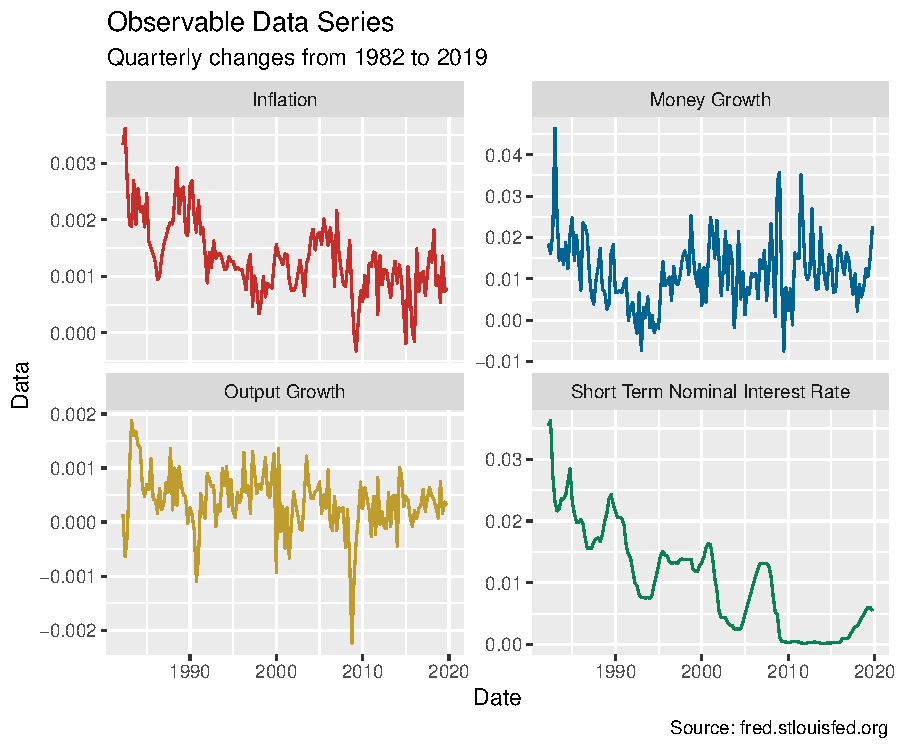
\includegraphics{Project_TS_20190565_files/figure-latex/unnamed-chunk-1-1.pdf}

\hypertarget{estimation}{%
\section{Estimation}\label{estimation}}

\hypertarget{calibration-and-priors}{%
\subsection{Calibration and Priors}\label{calibration-and-priors}}

To calibrate the model, I first calculated the logged first difference
of the quarterly data to get stationary series. The average values over
the entire sample period were calculated in order to obtain the
parameter values for inflation (\(\pi\)), interest rate (\(r\)) and
output growth (\(z\)). These values represent the steady state values as
we manipulated the data to capture changes from the steady state. Using
these values, the subjective discount rate (\(\beta\)) was calculated
using the following formula: \[ \beta = \Biggl(\frac{z}{r}\Biggl)\pi\]
Table \ref{tpar} below summarizes the parameter values that we calculate
using our data. The values are used when simulating the models for each
of the monetary rules.

\begin{table} 
\caption{Parameters calculater using own data}
\begin{center}
\begin{tabular}{ |c|c| } 
 \hline
 Parameter & Value \\ 
 \hline
 \(\pi\)& 1.00128 \\ 
  \(r\)& 1.00978  \\ 
  \(z\) & 1.00039 \\
  \(\beta\) & 0.99197 \\
 \hline
\end{tabular}
\label{tpar}
\end{center}
\end{table}

Figure \ref{fig:prior1} and Figure \ref{fig:prior2} plots the prior
distributions of the structural parameters, including the standard
deviations of the shocks. The five structural shocks: \(\sigma_a\),
\(\sigma_z\), \(\sigma_u\), \(\sigma_e\) and \(\sigma_r\) all have an
inverse chi-square distribution with four degrees of freedom.
\protect\hyperlink{ref-smets}{Smets \& Wouters}
(\protect\hyperlink{ref-smets}{2007}) argued in favour of rather lose
prior for the five shocks, and assigned the shocks inverse gamma
distributions with two degree of freedom. However,
\protect\hyperlink{ref-belongia2019reconsideration}{Belongia, Ireland \&
others} (\protect\hyperlink{ref-belongia2019reconsideration}{2019})
adjust this to allow the New Keynesian model to capture the increase in
volatility after the 2008/2009 financial crises.

\begin{table}
\caption{Exogenous Variables}
 \label{Table:enx}
 \begin{center}
\begin{tabular}{|c|c|} 
\hline
  Parameter & Description \\ 
\hline
 ${\sigma_a}$ & preference shock volatility\\
 ${\sigma_z}$ & productivity shock volatility\\
 ${\sigma_u}$ & money demand shock volatility\\
 ${\sigma_e}$ & cost push shock volatility\\
 ${\sigma_r}$ & monetary policy shock volatility\\
\hline
\end{tabular}
\end{center}
\end{table}

\begin{figure}
\caption{(a) Prior Distributions}
\centering
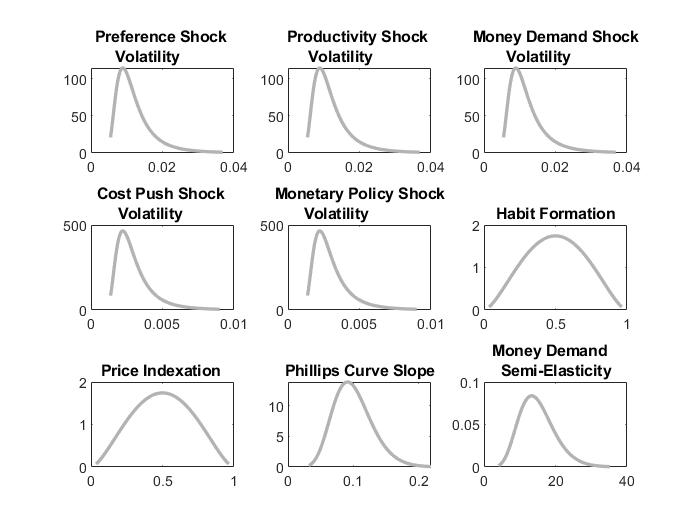
\includegraphics[scale=0.5]{prior.jpg}
\label{fig:prior1}
\end{figure}

\begin{figure}
\caption{(b) Prior Distributions}
\centering
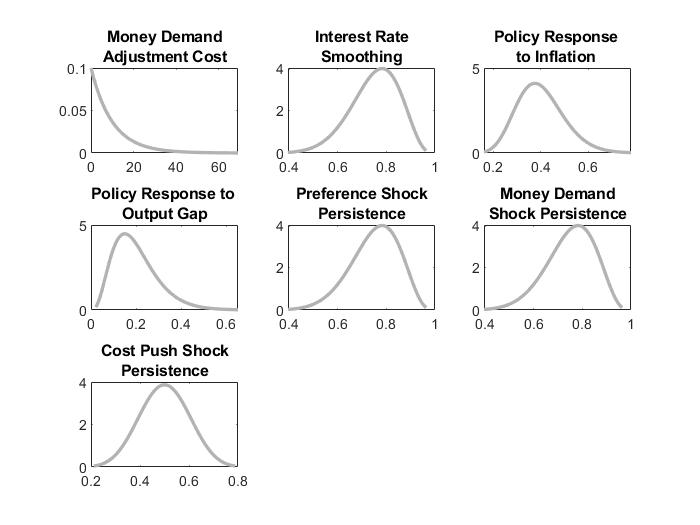
\includegraphics[scale=0.5]{prior_1.jpg}
\label{fig:prior2}
\end{figure}

Table \ref{Table:Prior} displays statistical characteristics of the
priors. The habit formation (\(\gamma\)) and price indexation
(\(\alpha\)) as well as the interest rate smoothing (\(\rho_r\)),
preference shock persistence (\(\rho_a\)), money demand shock
persistence (\(\rho_u\)) and cost push shock persistence (\(\rho_e\))
are constrained between zero and one by assigning a beta distribution to
the parameters. To restrict the parameters to positive values,
\protect\hyperlink{ref-belongia2019reconsideration}{Belongia, Ireland \&
others} (\protect\hyperlink{ref-belongia2019reconsideration}{2019})
assign gamma distributions for the Phillips curve slope (\(\psi\)),
money demand adjustment semi-elasticity (\(\delta_r\)), money demand
adjustment cost (\(\phi\)), policy response to inflation (\(\rho_\pi\))
and policy response to output gap (\(\rho_x\)).

\begin{table}
\caption{Prior information (parameters)}
 \label{Table:Prior}
 \begin{center}
\begin{tabular}{ |c|c|c|c|c|c|c|} 
\hline
  &  &  & & & \multicolumn{2}{|c|}{Bounds} \\ 
  \cline{6-7}
  Symbol & Description & Distribution & Mean & Std.dev. & Lower & Upper \\ 
\hline
$ {\sigma_a} $ & preference shock volatility & Inv. Chi-squared & 0.0125  & 0.0066 & 0.0000 & $\infty$  \\ 
$ {\sigma_z} $ & productivity shock volatility & Inv. Chi-squared  & 0.0125 & 0.0066 & 0.0000 & $\infty$ \\ 
$ {\sigma_u} $ & money demand shock volatility & Inv. Chi-squared & 0.0125  & 0.0066 & 0.0000 & $\infty$  \\ 
$ {\sigma_e} $ & cost push shock volatility & Inv. Chi-squared & 0.0031 & 0.0016 & 0.0000 & $\infty$  \\ 
$ {\sigma_r} $ & monetary policy shock volatility & Inv. Chi-squared & 0.0031  & 0.0016 & 0.0000 & $\infty$  \\ 
$ {\gamma} $ & habit formation& Beta & 0.5000  & 0.2000 & 0.0000 & 1.0000 \\ 
$ {\alpha} $ & price indexation  & Beta & 0.5000 & 0.2000 & 0.0000 & 1.0000  \\ 
$ {\psi} $ & Phillips curve slope & Gamma & 0.1000 & 0.0300 & 0.0000 & $\infty$ \\ 
$ {\delta_r} $ & money demand semi-elasticity & Gamma & 15.0000  & 5.0000 & 0.0000 & $\infty$ \\ 
$ {\phi} $ & money demand adjustment cost & Gamma & 10.0000 & 10.0000 & 0.0000 & $\infty$  \\ 
$ {\rho_r} $ & interest rate smoothing & Beta & 0.7500 & 0.1000 & 0.0000 & 1.0000 \\ 
$ {\rho_\pi} $ & policy response to inflation & Gamma & 0.4000  & 0.1000 & 0.0000 & $\infty$  \\ 
$ {\rho_x} $ & policy response to output gap & Gamma & 0.2000 & 0.1000 & 0.0000 & $\infty$ \\ 
$ {\rho_a} $ & preference shock persistence  & Beta & 0.7500  & 0.1000 & 0.0000 & 1.0000  \\ 
$ {\rho_u} $ & money demand shock persistence & Beta & 0.7500  & 0.1000 & 0.0000 & 1.0000  \\ 
$ {\rho_e} $ & cost push shock persistence & Beta & 0.5000  & 0.1000 & 0.0000 & 1.0000  \\ 
\hline
\end{tabular}
\end{center}
\end{table}

It is important to note that although the distribution for the shocks
are inverse chi-square, in the actual estimation, they are simulated as
having inverse gamma distribution. This is because the chi-square prior
is not implemented in \emph{dynare}. The chi-squared distribution is a
special case of the gamma distribution, therefore it is possible to
interchange between the two.

\hypertarget{posterior-estimation}{%
\subsection{Posterior Estimation}\label{posterior-estimation}}

Table \ref{tab_post} displays statistical information about the
posterior estimations for the Taylor rule and the flexible money growth
rate rule. The posterior mean and mode between the two rules are very
similar with the only noticeably large difference being the money demand
adjustment cost (\(\phi\)), where under the flexible money growth rate
rule it is twice as large. The standard deviation and the highest
posterior denisty interval (HPDI) upper and lower bound remain
relatively constant between the two rules, with, once again, the only
exception being money demand adjustment cost (\(\phi\)).

\begin{table}
\caption{Posterior Information - where HPD (L) and HPD (U) display the 90 percent Highest Posterior Density Interval Lower and Upper bound, respectively.}
 \begin{center}
\begin{tabular}{|c|c|c|c|c|c|c|c|c|}
\hline
\multicolumn{9}{|c|}{Taylor Rule} \\
\cline{1-9}
\hline
 &  & \multicolumn{2}{|c|}{Prior} & \multicolumn{5}{|c|}{Posterior}\\ 
  \cline{8-9}
\hline
  Symbol & Distribution & Mean & Std.dev. & Mean & Mode & Std. dev & HPD (L) & HPD (U)\\ 
\hline
$ {\sigma_a} $ & Inv. Chi-squared & 0.0125 & 0.0066  & 0.0694 & 0.0665 & 0.0215 & 0.0064 & 0.0237 \\ 
$ {\sigma_z} $ & Inv. Chi-squared  & 0.0125  & 0.0066  & 0.0086 & 0.0067 & 0.0019 & 0.0064 & 0.0237 \\ 
$ {\sigma_u} $ & Inv. Chi-squared & 0.0125  & 0.0066 & 0.0699 & 0.0336 & 0.0326 & 0.0064 & 0.0237 \\ 
$ {\sigma_e} $ & Inv. Chi-squared & 0.0031  & 0.0016 & 9.511e-04 & 7.294e-04  & 2.041e-04 & 0.0016 & 0.0058 \\ 
$ {\sigma_r} $ & Inv. Chi-squared & 0.0031  & 0.0016 & 0.0013 & 0.0013 & 8.628e-05 & 0.0016 & 0.0058 \\ 
$ {\gamma} $ & Beta & 0.5000  & 0.2000 & 0.9496 & 0.9383 & 0.0133 & 0.1718 & 0.8282 \\ 
$ {\alpha} $ & Beta & 0.5000 & 0.2000 & 0.9006 & 0.9655 & 0.0590 & 0.1718 & 0.8282 \\ 
$ {\psi} $ & Gamma & 0.1000  & 0.0300 & 0.0350  & 0.0108 & 0.0174 & 0.0563 & 0.1539 \\ 
$ {\delta_r} $ & Gamma & 15.0000 & 5.0000 & 12.5553  & 7.8858  & 5.7152 & 7.8254 & 24.0577 \\ 
$ {\phi} $ & Gamma & 10.0000 & 10.0000 & 36.3493 & 12.0157 & 21.4019 & 0.5129 & 29.9573 \\ 
$ {\rho_r} $ & Beta & 0.7500 & 0.1000 & 0.9079 & 0.8985 & 0.0216 &  0.5701 & 0.8971 \\ 
$ {\rho_\pi} $ & Gamma & 0.4000  & 0.1000  & 0.9836 & 0.8030 & 0.1464 & 0.2509 & 0.5774 \\ 
$ {\rho_x} $ & Gamma & 0.2000  & 0.1000 & 0.2909 & 0.2948 & 0.1080 & 0.0683 & 0.3877 \\ 
$ {\rho_a} $ & Beta & 0.7500 & 0.1000  & 0.9889 & 0.9905 & 0.0048 & 0.5701 & 0.8971 \\ 
$ {\rho_u} $ & Beta & 0.7500  & 0.1000 & 0.9642 & 0.9919 & 0.0289 & 0.5701 & 0.8971 \\ 
$ {\rho_e} $ & Beta & 0.5000  & 0.1000 & 0.5926 &  0.2348 & 0.2444& 0.3351 & 0.6649 \\ 
\hline
\multicolumn{9}{|c|}{Flexible Money Growth Rule} \\
\cline{1-9}
$ {\sigma_a} $ & Inv. Chi-squared & 0.0125 & 0.0066  & 0.0638 & 0.0716 & 0.0135 & 0.0462 & 0.0851\\ 
$ {\sigma_z} $ & Inv. Chi-squared  & 0.0125  & 0.0066 & 0.0051 & 0.0046 &  4.604e-04 & 0.0043 & 0.0058 \\ 
$ {\sigma_u} $ & Inv. Chi-squared & 0.0125  & 0.0066 & 0.0073 & 0.0066 & 0.0015 & 0.0048 & 0.0094\\ 
$ {\sigma_e} $ & Inv. Chi-squared & 0.0031  & 0.0016 & 6.414e-04 & 635e-04 & 3.969e-05 &  5.760e-04 & 7.031e-04\\ 
$ {\sigma_r} $ & Inv. Chi-squared & 0.0031  & 0.0016 & - & - & - & - & -\\ 
$ {\gamma} $ & Beta & 0.5000  & 0.2000 & 0.9132 & 0.9055 & 0.0114 & 0.8931 & 0.9304 \\ 
$ {\alpha} $ & Beta & 0.5000 & 0.2000 & 0.8475 &  0.8436 & 0.0397 & 0.7789 & 0.9076\\ 
$ {\psi} $ & Gamma & 0.1000  & 0.0300 & 0.0038 & 0.0046 & 9.218e-04 & 0.0024 & 0.0054 \\ 
$ {\delta_r} $ & Gamma & 15.0000 & 5.0000 & 8.6681 & 8.1955 & 1.0702 & 6.9422 & 10.4597\\ 
$ {\phi} $ & Gamma & 10.0000 & 10.0000 & 68.35 & 65.6454 & 16.5853 & 39.4357 & 95.0324\\ 
$ {\rho_r} $ & Beta & 0.7500 & 0.1000 & 0.7637 & 0.7817 & 0.0886 & 0.6258 & 0.9141\\ 
$ {\rho_\pi} $ & Gamma & 0.4000  & 0.1000 & 0.3970 & 0.3750 & 0.0964 & 0.2480 & 0.5210\\ 
$ {\rho_x} $ & Gamma & 0.2000  & 0.1000 & 0.2003 & 0.1500 & 0.0939 & 0.0484 & 0.3420\\ 
$ {\rho_a} $ & Beta & 0.7500 & 0.1000  &  0.9902 & 0.9920 & 0.0019 & 0.9876 & 0.9932\\ 
$ {\rho_u} $ & Beta & 0.7500  & 0.1000 & 0.8574 & 0.8548 & 0.0496 & 0.7652 & 0.9277\\ 
$ {\rho_e} $ & Beta & 0.5000  & 0.1000 & 0.1189 & 0.1263 & 0.0247 & 0.0786 & 0.1579 \\ 
\hline
\end{tabular}
\end{center}
\label{tab_post}
\end{table}

\hypertarget{mcmc-acceptance-ratio}{%
\subsection{MCMC acceptance ratio}\label{mcmc-acceptance-ratio}}

Since the DSGE model specified has more than five parameters, we would
expect to see an acceptance ration of around 23 percent
\protect\hyperlink{ref-bedard2008optimal}{Bedard}
(\protect\hyperlink{ref-bedard2008optimal}{2008}). In my \emph{dynare}
code, I set the number of Metropolis-Hastings Chains to two, which is
the default and the number of iteration to 25 000. The acceptance ratios
are all strictly positive and close the expected value. The Taylor rule
and constant money growth rule are slightly above the expected average,
and the flexible money growth rate rule acceptance ratio is slightly
below.

\begin{table}
\caption{MCMC acceptance ratio (precent)}
 \label{mcmc_acceptance}
 \begin{center}
\begin{tabular}{|c|c|c|c|} 
\hline
   & Taylor Rule & Flexible Money Growth rate Rule & Constant Money Growth Rule \\ 
\hline
 Chain 1 & 31.184 & 18.616 & 33.192 \\
 Chain 2 & 35.176 & 17.228 & 33.784 \\
\hline
\end{tabular}
\end{center}
\end{table}

\hypertarget{blanchard-khan-stability-conditions}{%
\subsection{Blanchard-Khan Stability
Conditions}\label{blanchard-khan-stability-conditions}}

The assumption that macroeconomic models assume perfect foresight has
been widely critiqued. However, the assumption has been made possible
due to improvement of simulation algorithms. For the model to have a
unique solution, the Blanchard-Khan conditions have to be met. These
conditions are easy to check, in terms of eigenvalues computed at the
steady state of the model
\protect\hyperlink{ref-laffargue2000blanchard}{Laffargue \& others}
(\protect\hyperlink{ref-laffargue2000blanchard}{2000}). This unique
solution for the model is determined if and only if the number of
unstable eigenvalues is equal to the number of non-predetermined
variables. The Blanchard-Khan condition for the DSGE model of this
project is satisfied as there are five eigenvalues larger than one in
the modulus for five forward looking variables in the model.

\hypertarget{bayesian-impulse-response-functions}{%
\subsection{Bayesian Impulse Response
functions}\label{bayesian-impulse-response-functions}}

Much research in macroeconomics have been done to understand the
relative impact of different shock on aggregate economic activity.
Analyzing the bayesian Impulse response functions, the Taylor rule seems
to deliver better results given a shock to preferences and productivity,
while the flexible money growth rule delivers similar-to-better results
for the money demand and cost push shocks. The IRFs that we simulated
look very similar to
\protect\hyperlink{ref-belongia2019reconsideration}{Belongia, Ireland \&
others} (\protect\hyperlink{ref-belongia2019reconsideration}{2019}) in
shape.

The gray shaded area reflects the highest posterior density interval
(HPDI). A description of the variables can be found in table
\ref{Table:end} under appendix A.

\hypertarget{preference-shock}{%
\subsubsection{Preference Shock}\label{preference-shock}}

Figure \ref{tay_a} and Figure \ref{flex_a} represents the impulse
response functions as a results of a preference shock to the variables
in the model for the Taylor rule and the flexible money growth rule,
respectively. Preference shock can be interpreted as a shock to
household production, since it will affect household behaviour by
affecting savings-consumption decisions.

A positive preference shock leads to an increase in labour supply and
decrease in leisure, which in turn leads to an increase in initial
output and consumption. Consequently, we would expect to see that
savings and investment decrease. After prices and wages adjust, the
output growth slowly returns to its steady state.

In figure \ref{tay_a} and Figure \ref{flex_a}, an initial spike in
inflation can be seen. This is due to the increase in output and labour
supply. However, inflation returns to its steady state faster under the
Taylor rule. The Taylor rule and the flexible monetary policy growth
rule have similar responses, with the flexible monetary policy rule
being more volatile to changes in output gap (\(x\)) and money growth
(\(\mu\)) and therefore taking longer to return to its steady states
values.

\begin{figure}
    \centering 
    \begin{minipage}[t]{8.2cm} 
        \centering 
        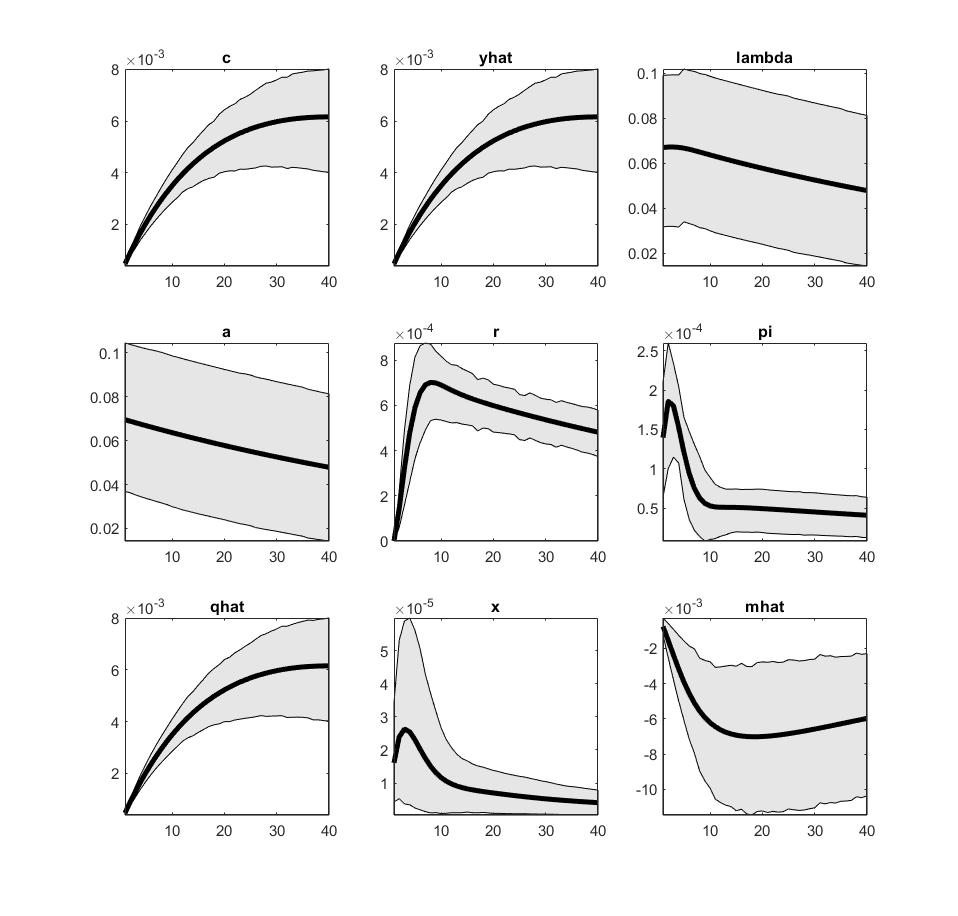
\includegraphics[width=\linewidth]{tay_a1.jpg} 
    \end{minipage} 
    \hspace{0.1cm} 
    \begin{minipage}[t]{8.2cm} 
        \centering 
        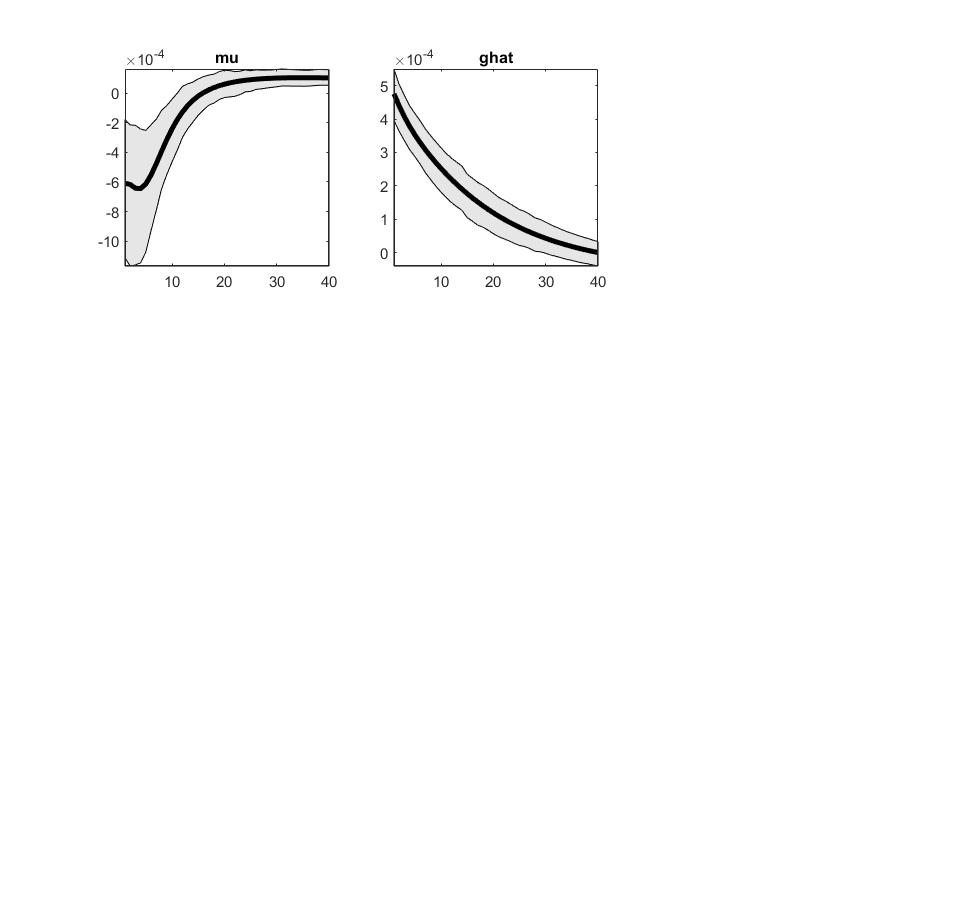
\includegraphics[width=\linewidth]{tay_a2.jpg} 
    \end{minipage}
    \caption{Orthogonalized Shock to Preference Shock - Taylor Rule}
    \label{tay_a}
\end{figure}

\begin{figure}
    \centering 
    \begin{minipage}[t]{8.2cm} 
        \centering 
        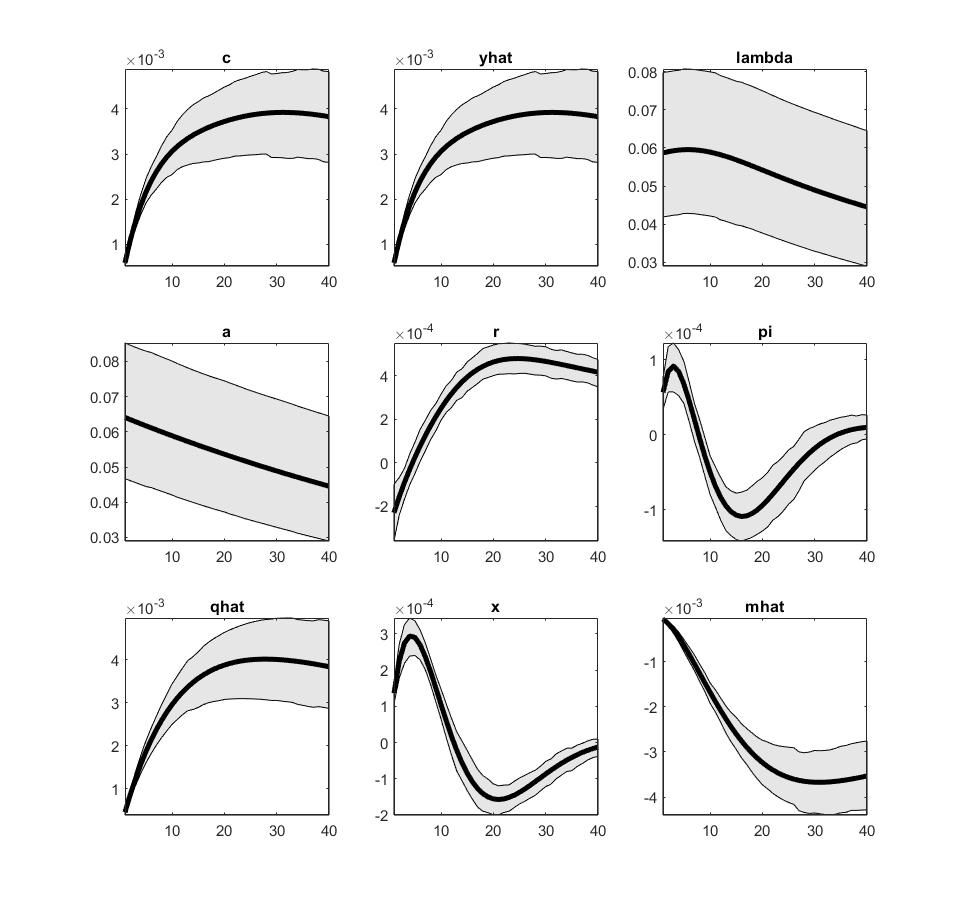
\includegraphics[width=\linewidth]{flex_a1.jpg} 
    \end{minipage} 
    \hspace{0.1cm} 
    \begin{minipage}[t]{8.2cm} 
        \centering 
        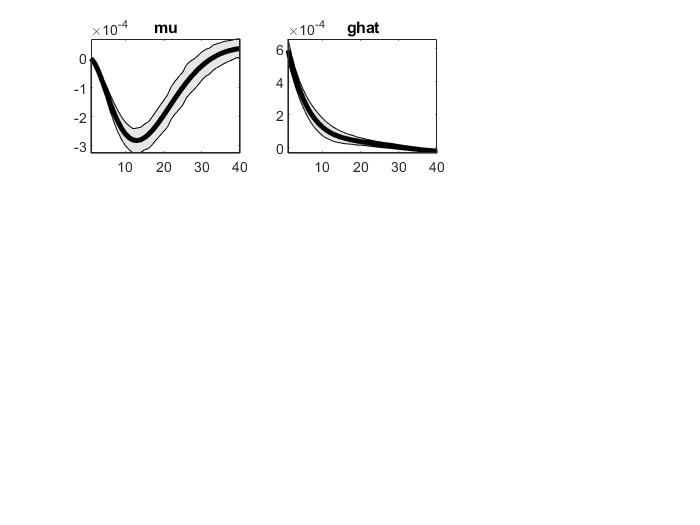
\includegraphics[width=\linewidth]{flex_a2.jpg} 
    \end{minipage}
    \caption{Orthogonalized Shock to Preference Shock - Flexible Money Growth Rule}
    \label{flex_a}
\end{figure}

\hypertarget{productivity-shock-z}{%
\subsubsection{Productivity Shock (z)}\label{productivity-shock-z}}

Figure \ref{tay_z} and Figure \ref{flex_z} represents the impulse
response functions as a results of a productivity shock to the variables
in the model for the Taylor rule and the flexible money growth rule,
respectively. A positive productivity shock is expected to persist over
time, although not permanently. Therefore, a productivity shocks leads
to an increase in hours worked and real wage which in turn increase
output, consumption and investment. The increase in output would then
lead to an increase in money growth, as it would be necessary to
increase money printing.

The flexible money growth rules better reflects what we theoretically
would expect to see when a productivity shock occurs. Figure \ref{tay_z}
and \ref{flex_z} support the view that productivity shocks play an
important roles in accounting for fluctuations in output. Furthermore,
it supports the view that technology shocks affect the marginal product
of labour and the marginal product of capital.

\begin{figure}
\centering
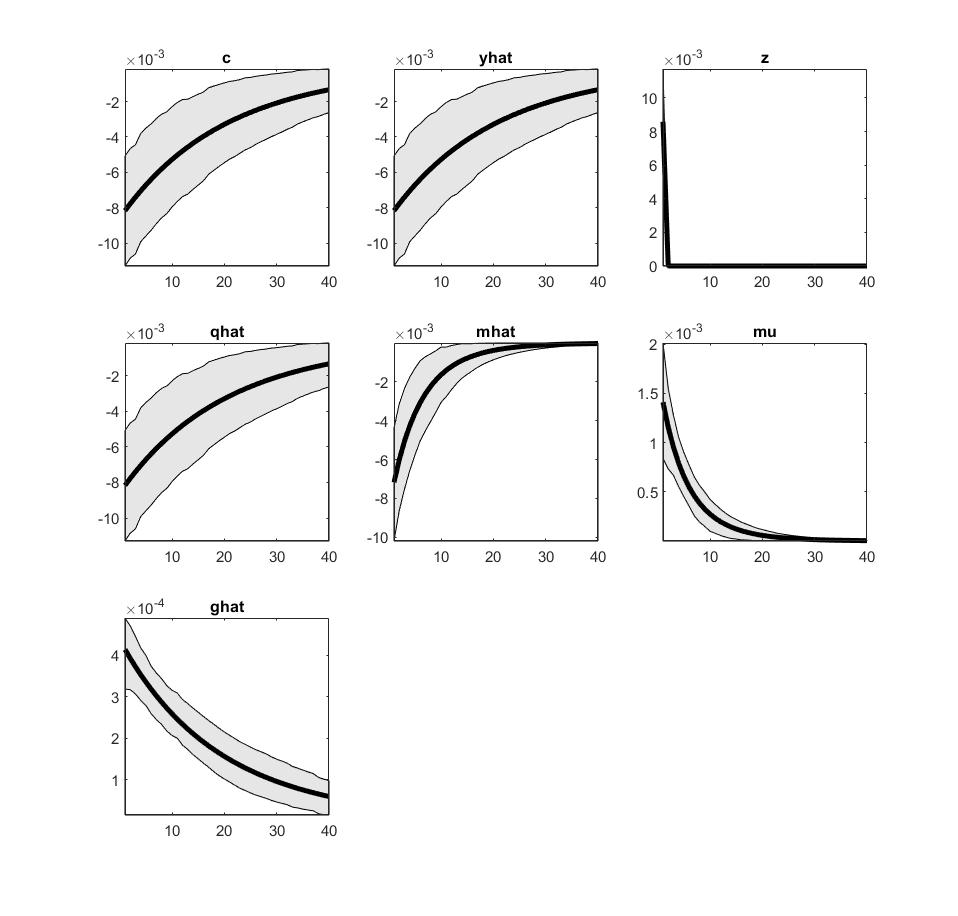
\includegraphics[scale=0.3]{tay_z.jpg}
\caption{Orthogonalized Shock to Productivity Shock - Taylor Rule}
\label{tay_z}
\end{figure}

\begin{figure}
    \centering 
    \begin{minipage}[t]{8.2cm} 
        \centering 
        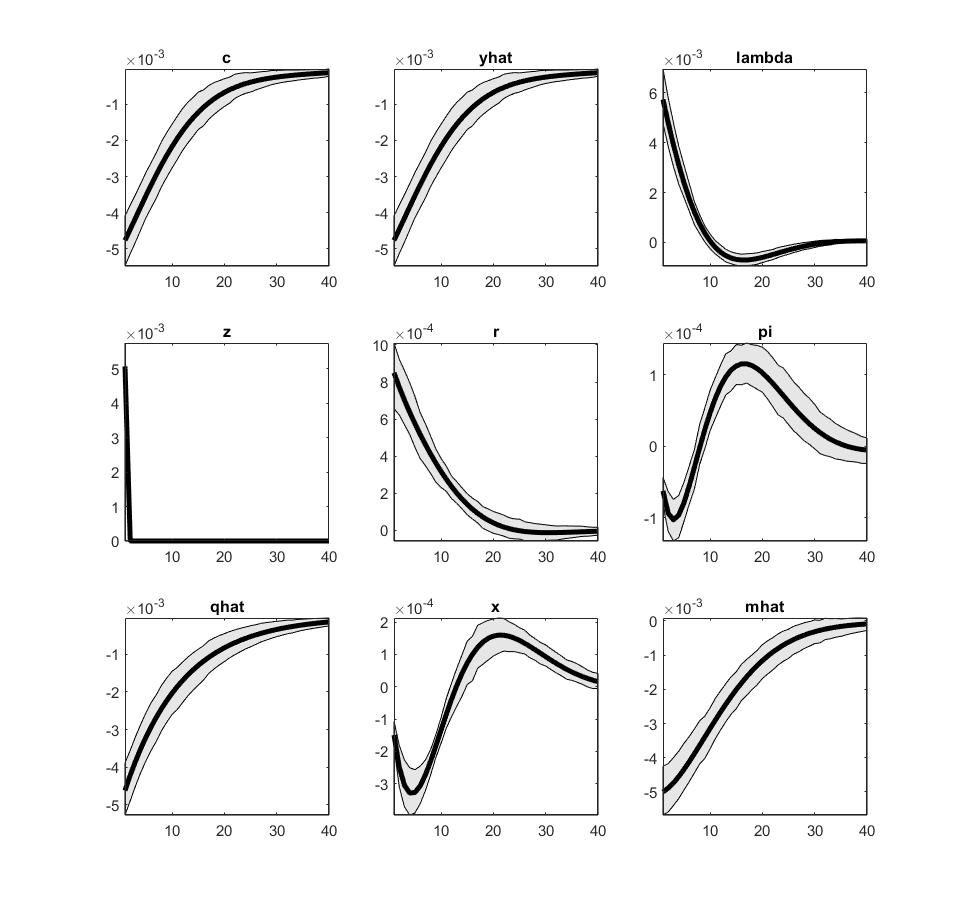
\includegraphics[width=\linewidth]{flex_z1.jpg} 
    \end{minipage} 
    \hspace{0.1cm} 
    \begin{minipage}[t]{8.2cm} 
        \centering 
        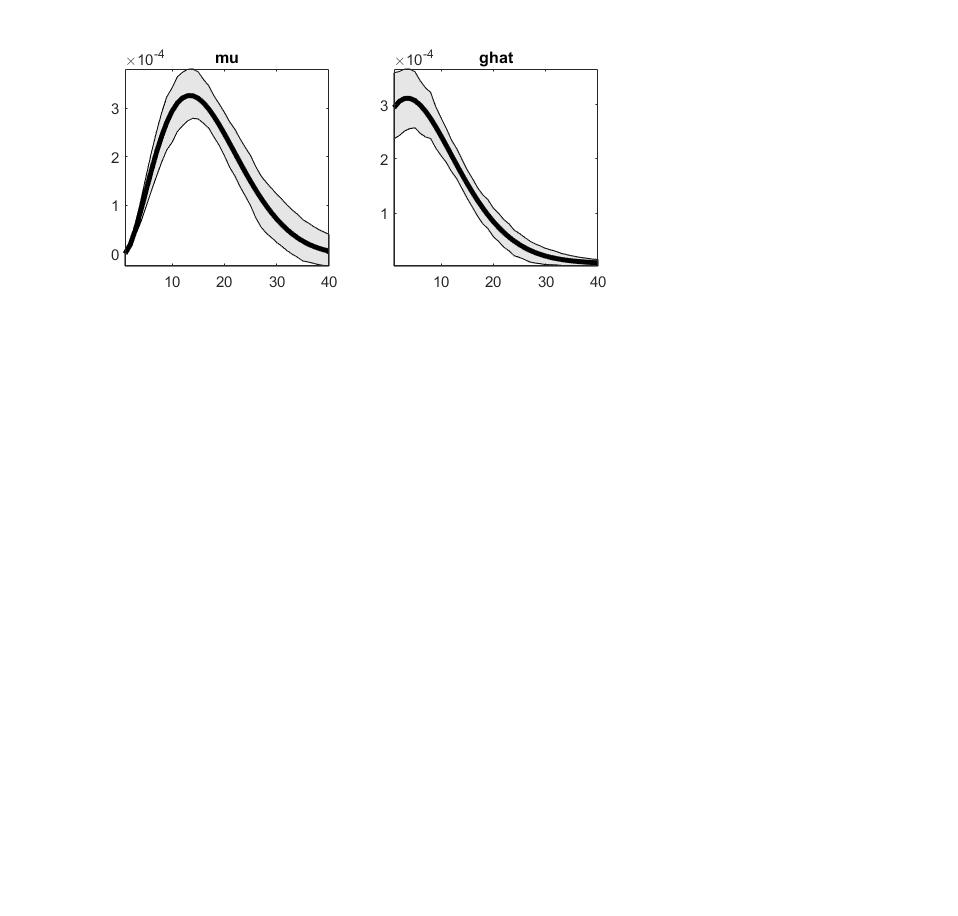
\includegraphics[width=\linewidth]{flex_z2.jpg} 
    \end{minipage}
    \caption{Orthogonalized Shock to Productivity Shock - Flexible Money Growth Rule}
    \label{flex_z}
\end{figure}

\hypertarget{money-demand-shock-u}{%
\subsubsection{Money Demand Shock (u)}\label{money-demand-shock-u}}

Figure \ref{tay_u} and Figure \ref{flex_u} represents the impulse
response functions as a results of a money demand shock to the variables
in the model for the Taylor rule and the flexible money growth rule,
respectively. Money demand shocks are more likely to lead to volatility
in inflation and output. This results can be seen in figure
\ref{flex_u}, which shows that output (\(\hat{y}\)), consumption
(\(c\)), inflation (\(\pi\)), output gap (\(x\)) and money growth
(\(\mu\)) all follow volatility and similar paths. The rise in the
demand for money is temporarily followed by an increase in the growth
rate of money (\(\mu\)), which in turn exerts upward pressure on
inflation (\(\pi\)), as can be seen in in figure \ref{flex_u}.

\begin{figure}
\centering
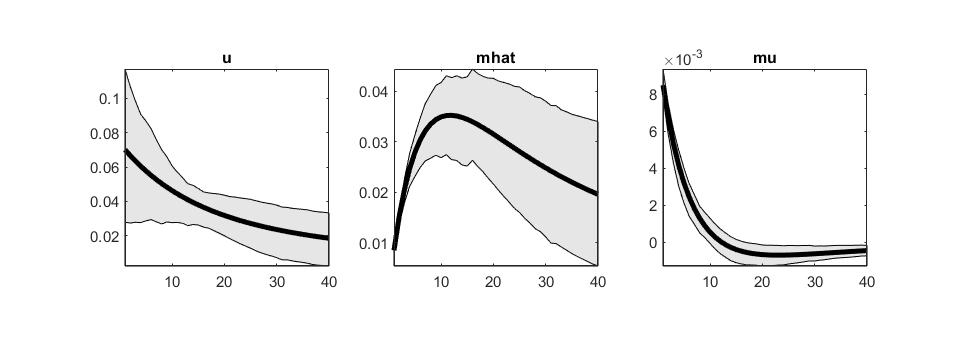
\includegraphics[scale=0.5]{tay_u.jpg}
\caption{Orthogonalized Shock to Money Demand Shock - Taylor Rule}
\label{tay_u}
\end{figure}

\begin{figure}
    \centering 
    \begin{minipage}[t]{8.2cm} 
        \centering 
        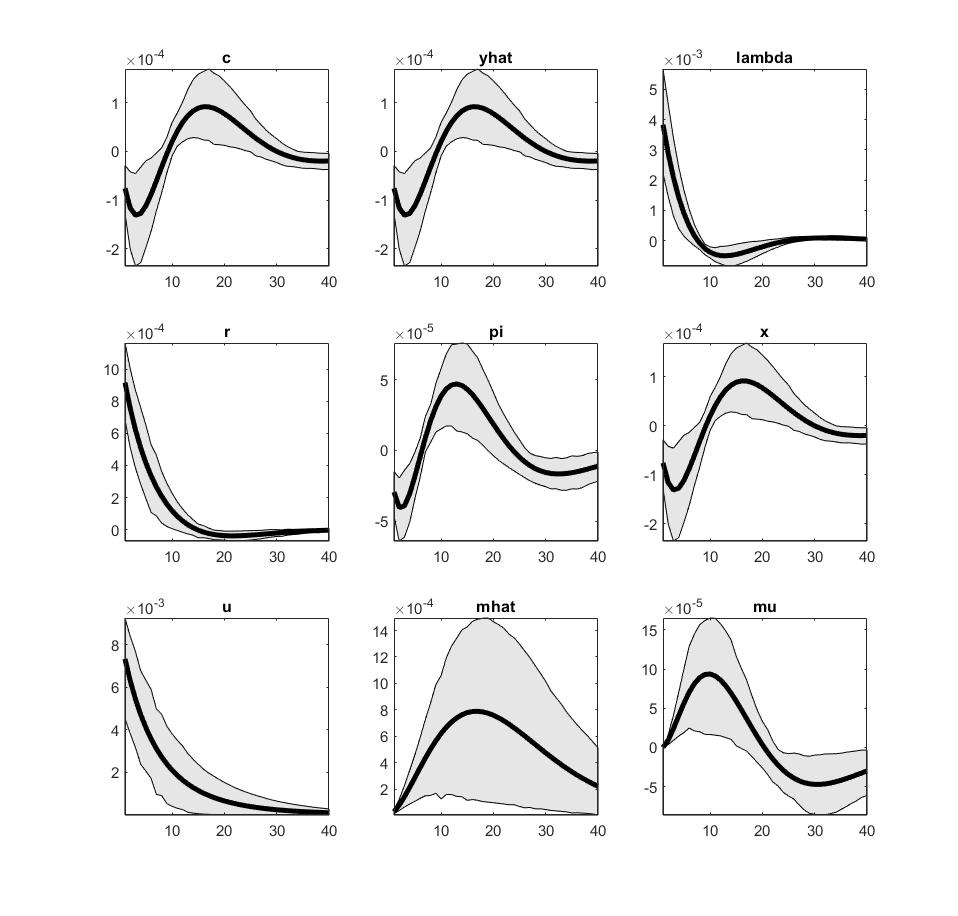
\includegraphics[width=\linewidth]{flex_u1.jpg} 
    \end{minipage} 
    \hspace{0.1cm} 
    \begin{minipage}[t]{8.2cm} 
        \centering 
        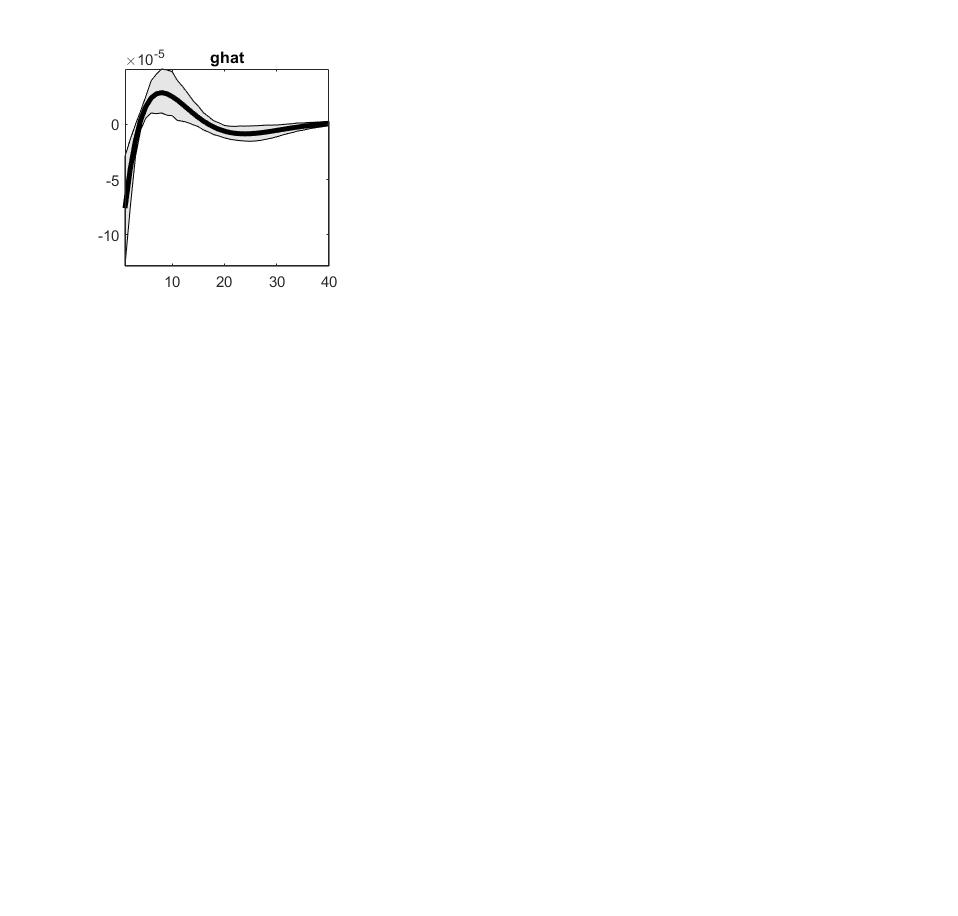
\includegraphics[width=\linewidth]{flex_u2.jpg} 
    \end{minipage}
    \caption{Orthogonalized Shock to Money Demand Shock - Flexible Money Growth Rule}
    \label{flex_u}
\end{figure}

\hypertarget{cost-push-shock-e}{%
\subsubsection{Cost Push Shock (e)}\label{cost-push-shock-e}}

Cost push shocks are transitory deviations between the flexible price
equilibrium and efficient allocation. Cost push shocks create a increase
in inflation and a decrease in output gap, simultaneous. Therefore, the
optimal response of the central bank is extremely controversial. The
central bank can make one of two contradicting choices; it can either
relax its monetary policy in order to accommodate the negative output
gap, or it can tighten its monetary policy in order to combat the
increase inflation. Figure \ref{tay_e} and Figure \ref{flex_e}
represents the impulse response functions as a results of a cost push
shock to the variables in the model for the Taylor rule and the flexible
money growth rule, respectively.

The Taylor rule and the flexible money growth rate rule are
comparatively similar. This implies that the flexible money growth rate
rule can be used as an alternative to the Taylor rule give most of the
shocks.

\begin{figure}
    \centering 
    \begin{minipage}[t]{8.2cm} 
        \centering 
        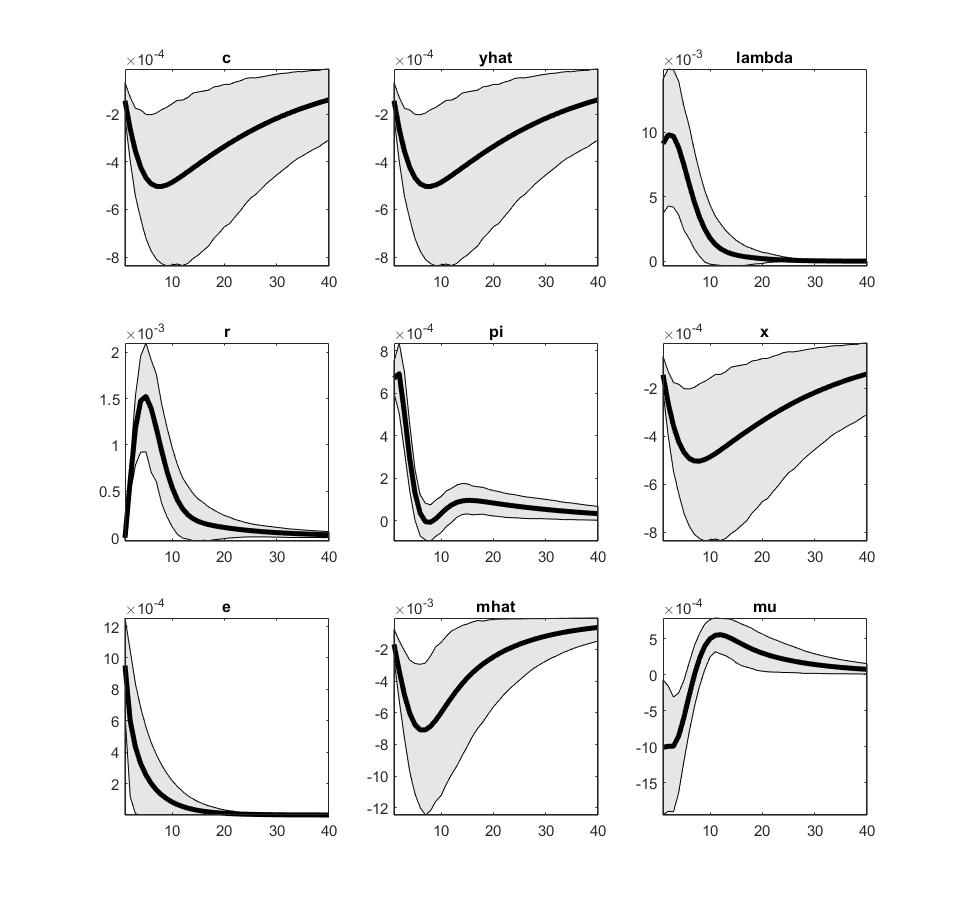
\includegraphics[width=\linewidth]{tay_e1.jpg} 
    \end{minipage} 
    \hspace{0.1cm} 
    \begin{minipage}[t]{8.2cm} 
        \centering 
        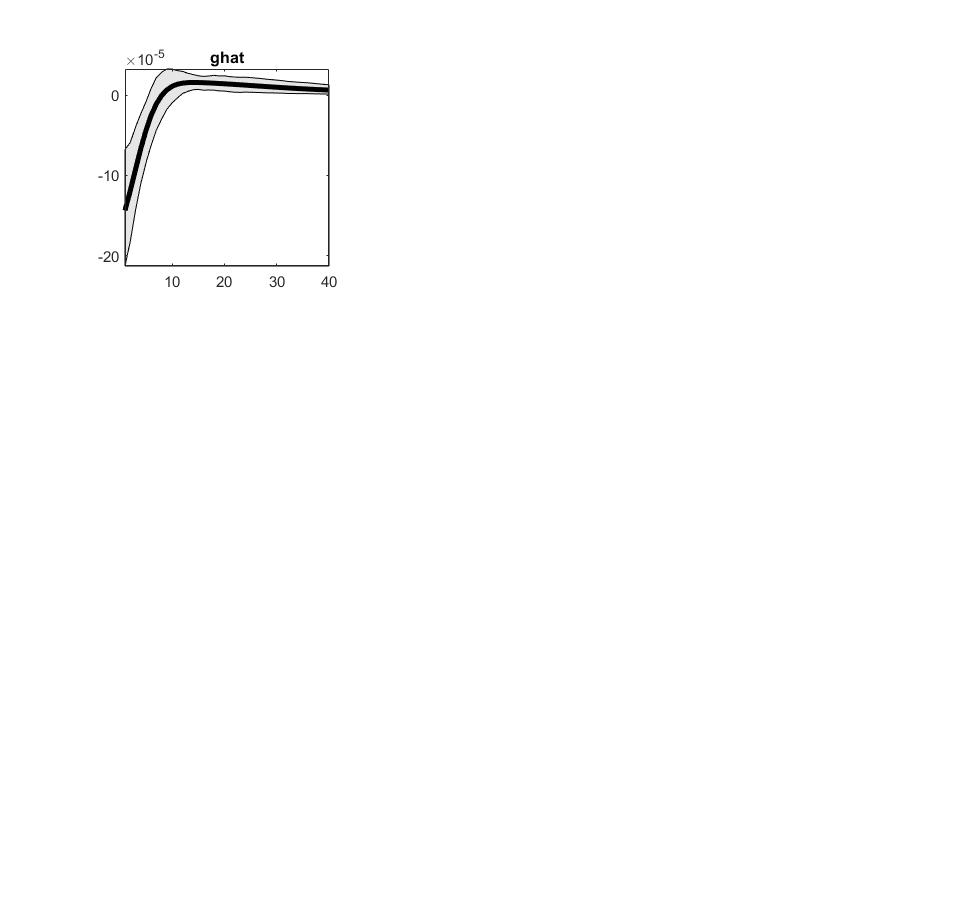
\includegraphics[width=\linewidth]{tay_e2.jpg} 
    \end{minipage}
    \caption{Orthogonalized Shock to Cost Push Shock - Taylor Rule}
    \label{tay_e}
\end{figure}

\begin{figure}
    \centering 
    \begin{minipage}[t]{8.2cm} 
        \centering 
        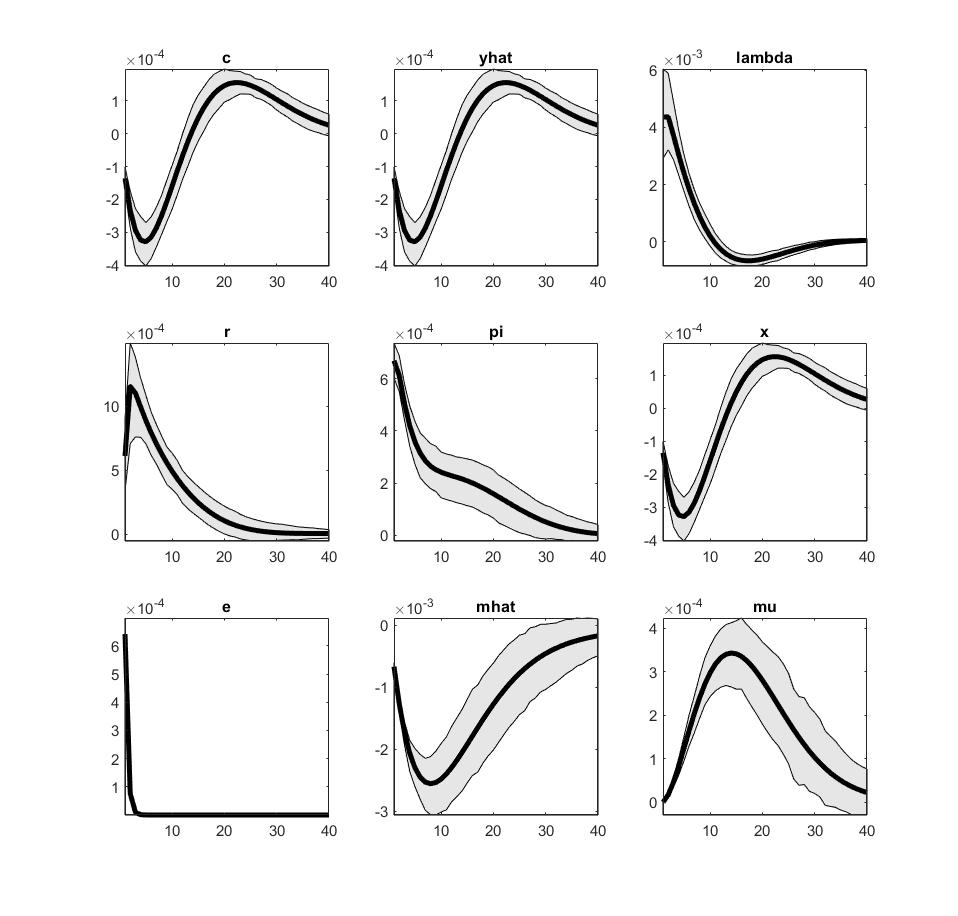
\includegraphics[width=\linewidth]{flex_e1.jpg} 
    \end{minipage} 
    \hspace{0.1cm} 
    \begin{minipage}[t]{8.2cm} 
        \centering 
        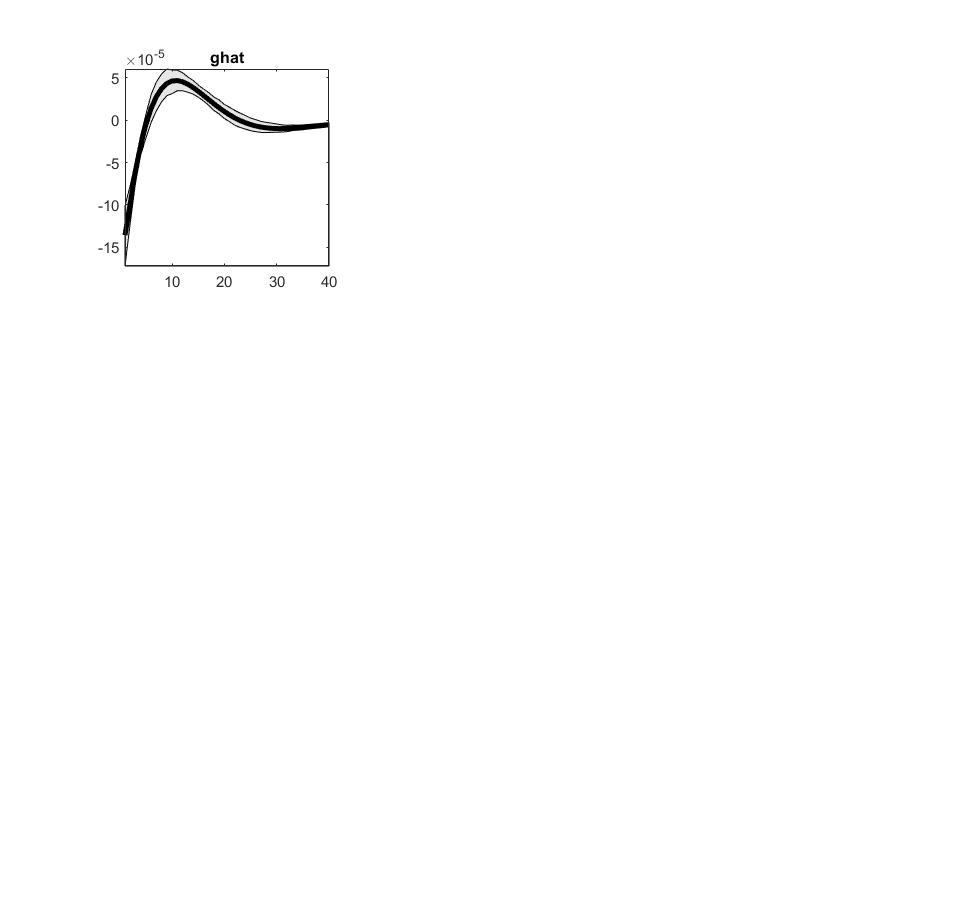
\includegraphics[width=\linewidth]{flex_e2.jpg} 
    \end{minipage}
    \caption{Orthogonalized Shock to Cost Push Shock - Flexible Money Growth Rule}
    \label{flex_e}
\end{figure}

\hypertarget{evaulation}{%
\section{Evaulation}\label{evaulation}}

Many resources and time has been dedicated to find the optimal rule to
advise monetary policy rules. An optimal monetary policy rule is
designed in such a manner as to stabilize prices and output as well as
boost consumer confidence. In this section, several diagnostic test are
carried out in order to analyze the empirical fit of the DSGE model in
terms of the Taylor rule and the flexible money growth rule. The Taylor
rule and flexible money growth rule will be analyzed and compared, with
some reference being made to the constant money growth rule.

\hypertarget{mode-plots}{%
\subsection{Mode Plots}\label{mode-plots}}

Figure \ref{mode_tay} and \ref{mode_flex} display the mode check plots
for the taylor rule and the flexible money growth rule, respectively.
The difference in the shapes of the likelihood kernel (red line) and the
posterior likelihood (blue line) indicates the role of the prior in
influencing the curvature of the likelihood function. As can be seen in
the plots, the mode is at the maximum point of the posterior likelihood.
This implies that there are no identification problems. The red dots on
the figures indicates a violation of the Blanchard-Kahn conditions and
the model could not solve those parameter values.

There are slight difference between the taylor rule and the flexible
money growth rule mode check plots. These differences are due to the
observed money growth being included in the taylor rule but not the
flexible money growth rate rule.

\begin{figure}
    \centering 
    \begin{minipage}[t]{8.2cm} 
        \centering 
        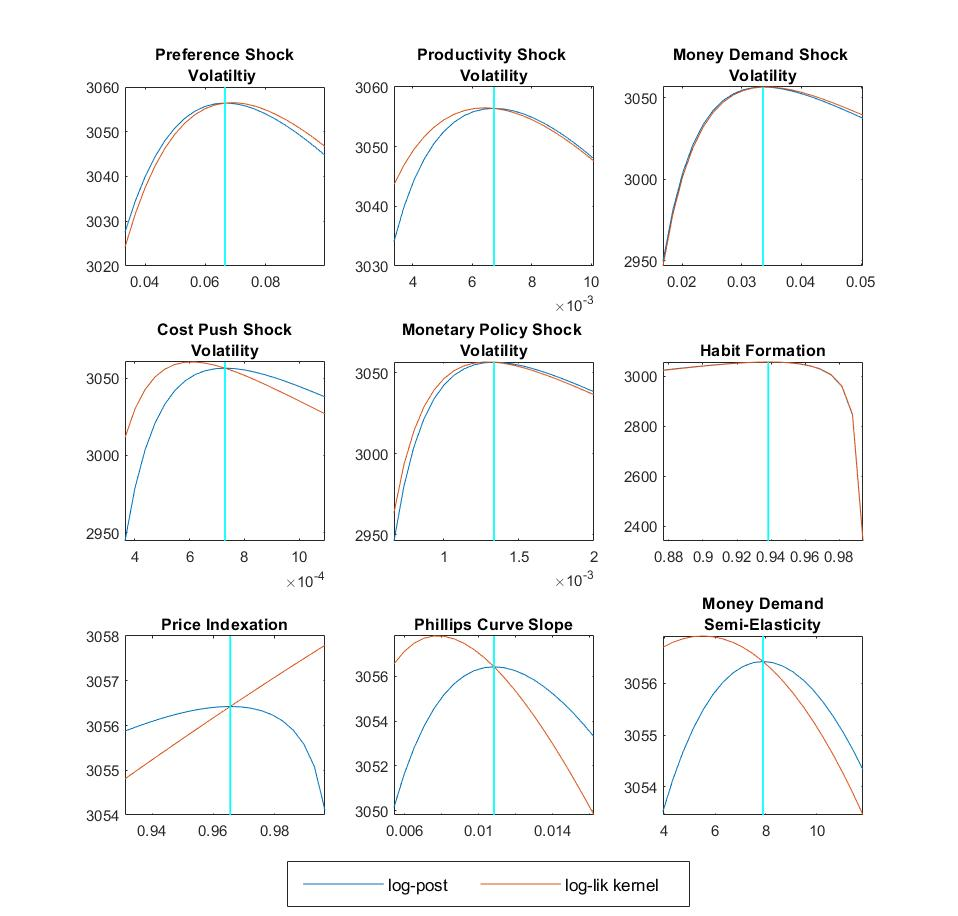
\includegraphics[width=\linewidth]{taylor.jpg} 
    \end{minipage} 
    \hspace{0.1cm} 
    \begin{minipage}[t]{8.2cm} 
        \centering 
        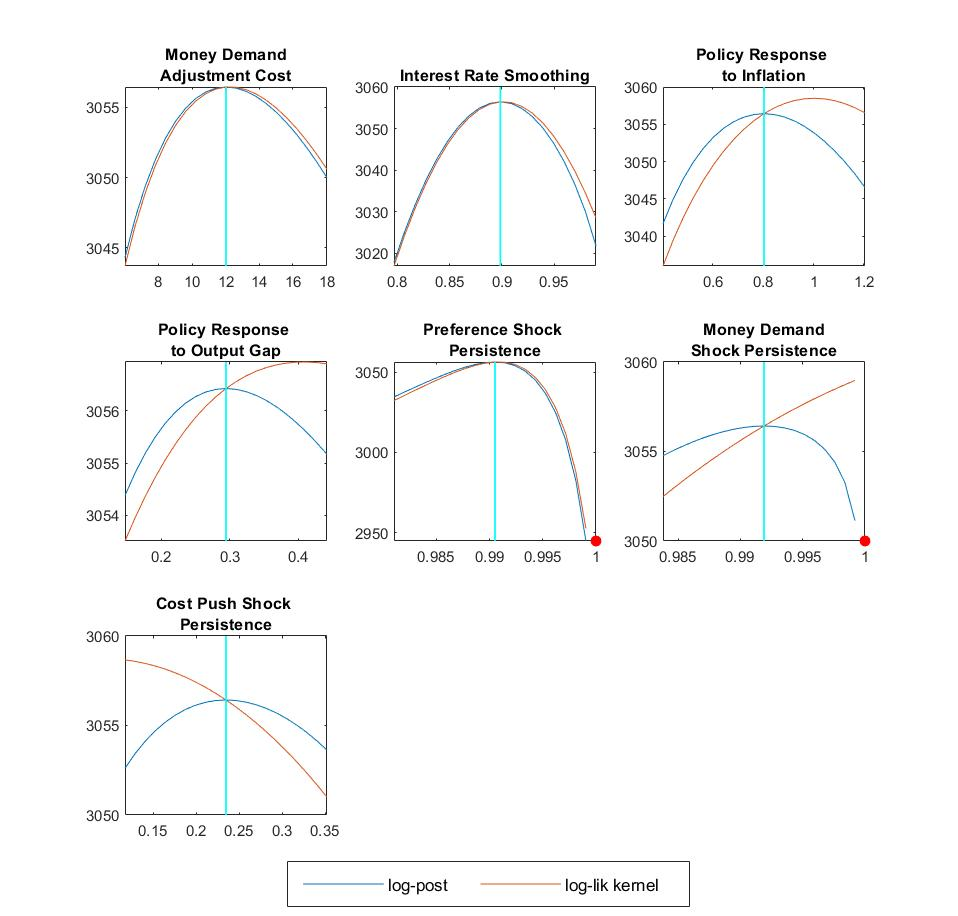
\includegraphics[width=\linewidth]{taylor1.jpg} 
    \end{minipage}
    \caption{Mode Check Plots - Taylor Rule}
    \label{mode_tay}
\end{figure}

\begin{figure}
    \centering 
    \begin{minipage}[t]{8.2cm} 
        \centering 
        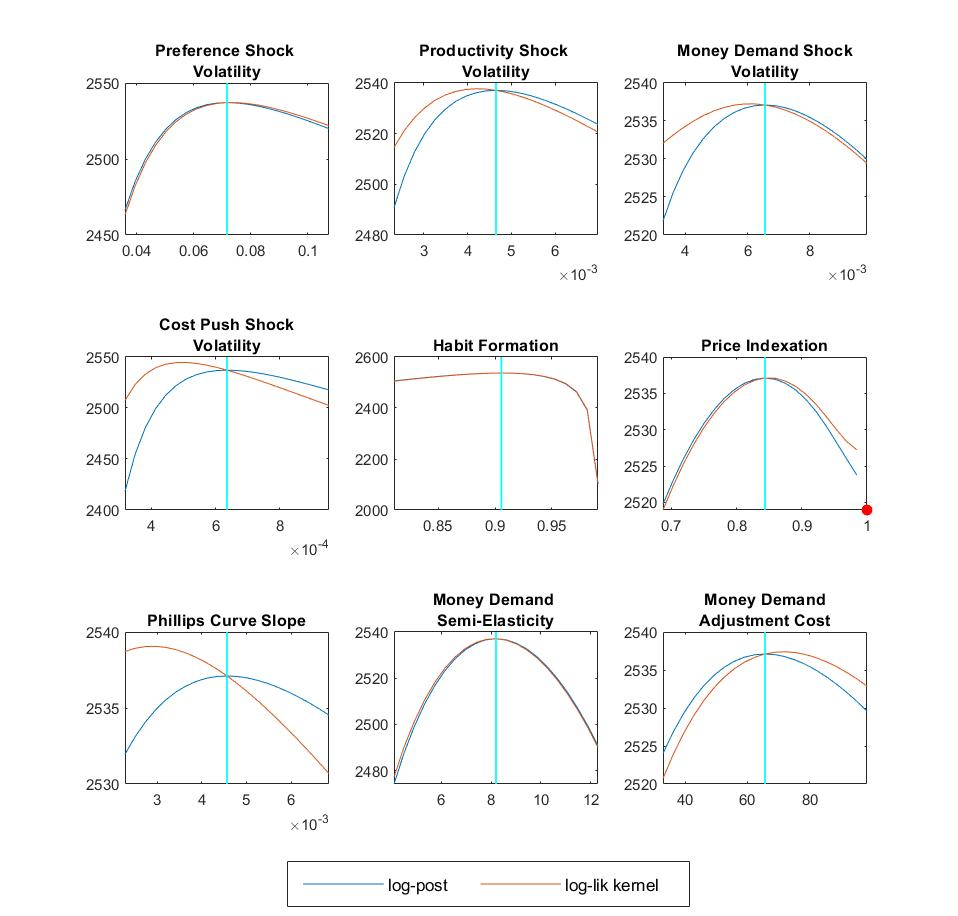
\includegraphics[width=\linewidth]{flex.jpg} 
    \end{minipage} 
    \hspace{0.1cm} 
    \begin{minipage}[t]{8.2cm} 
        \centering 
        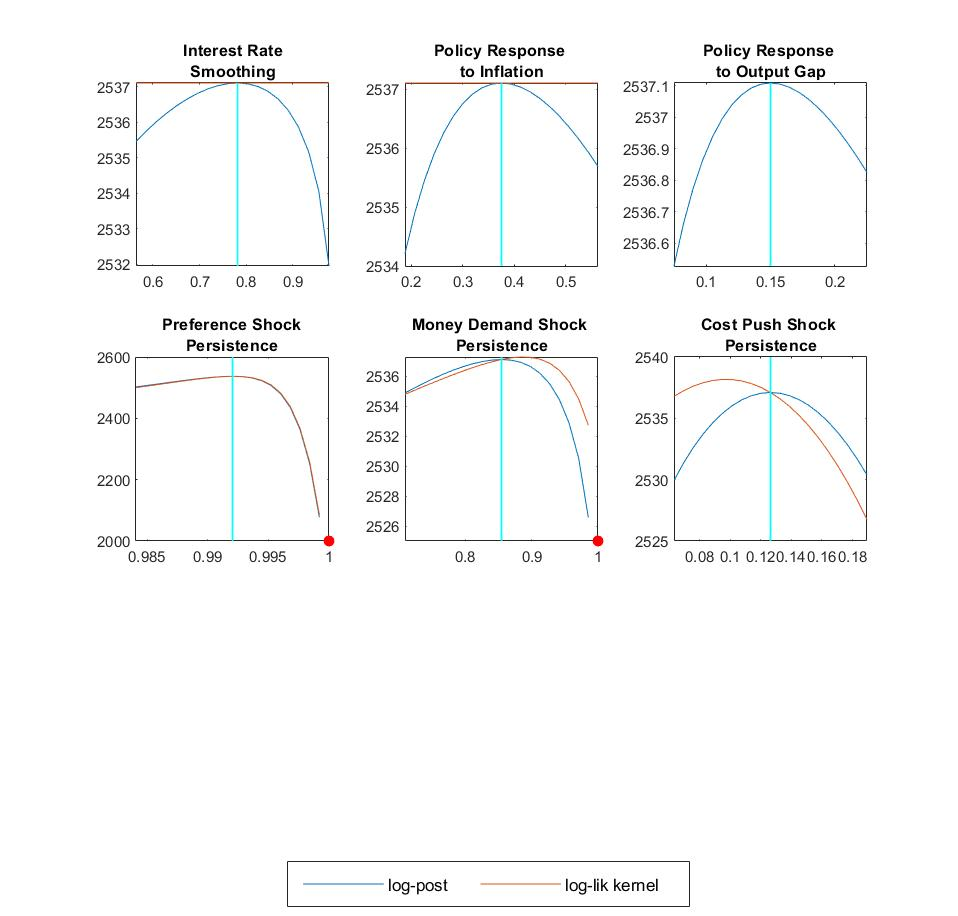
\includegraphics[width=\linewidth]{flex1.jpg} 
    \end{minipage}
    \caption{Mode Check Plots - Flexible Money Growth Rule}
    \label{mode_flex}
\end{figure}

\hypertarget{monte-carlo-markov-chain-univariate-diagnostics}{%
\subsection{Monte Carlo Markov Chain univariate
diagnostics}\label{monte-carlo-markov-chain-univariate-diagnostics}}

It is extremely challenging to test for the convergence of the posterior
distribution. However, \emph{dynare} provides us with Monte Carlo Markov
Chain (MCMC) univariate diagnostics which makes it easier to analyze.
Figure \ref{mcmctay}, \ref{mctay12}, \ref{mctay34} and \ref{mctay56} as
well as figure \ref{mcflex}, \ref{mcflex12}, \ref{mcflex34},
\ref{mcflex5} represents convergences indicators for all parameters
considered for the Taylor rule and the flexible money growth rule.

There are three plots for each parameter. The first plot shows the
convergence diagnostics for the 80 percent interval. The second plot
shows the estimate of the second central moment (m2), the variance, and
the third plot shows the estimate of the third central moment (m3). The
red line shows the 80 percent quantile range based on the pooled draws
from all sequences and the blue line shows the mean interval range based
on the draws of the individual sequences. The plots can be interpreted
as the chains having converged if the red and blue line stabilize
horizontally and remain close to each other.

I expect to see that many of the iterations of the Metropolis-Hasting
simulating to be similar, meaning that for the results to be sensible, I
would expect to see the red and blue lines remain relatively constant
and they should converge. Studying the results for the Taylor rule, I
find mixed results. Preference shock volatility (\(\sigma_a\)),
productivity shock volatility (\(\sigma_z\)), monetary policy shock
volatility (\(\sigma_r\)), price indexation (\(\alpha\)), Interest rate
smoothing (\(\rho_r\)), policy response to inflation (\(\rho_\pi\)),
policy response to output gap (\(\rho_x\)) and preference shock
persistence (\(\rho_a\)) all seem to all converge, especially in
relation \emph{interval}. However, the other eight variables show
greater variation during the process of convergence. This unsatisfactory
performance for the estimation of these parameters is related to the
prior values for each as they show weak identification. This is
concerning since the the general results displayed in figure
\ref{mcmctay} is considered unsatisfactory, implying that the prior
might need reconsideration. Figure \ref{mcmctay} also shows that the
parameters converge to the target distribution at around 10 000
iterations, after which they drastically diverge again.

However, the flexible money growth rate rule shows much more promising
and satisfactory results. The only parameter that does not converge is
the preference shock persistence (\(\rho_a\)). The results are extremely
satisfactory, implying that that is no reasons to change the prior
values. Figure \ref{mccon} shows that the general results for the
constant money growth rule is similar to that of the flexible money
growth rate rule, however, it seems to diverge at 4000 iterations before
it converges again at 7000 iterations. The divergence implies that the
flexible money growth rate is more stable than the constant money growth
rate. This suggest that the flexible money growth rule could lead to a
more stable and predicable path of the parameters. Thus, taking only the
MCMC univariate diagnostics into account, I conclude that the flexible
Money growth rule is more optimal given the information in the observed
data.

\begin{figure}
\caption{MCMC general - Taylor Rule}
\centering
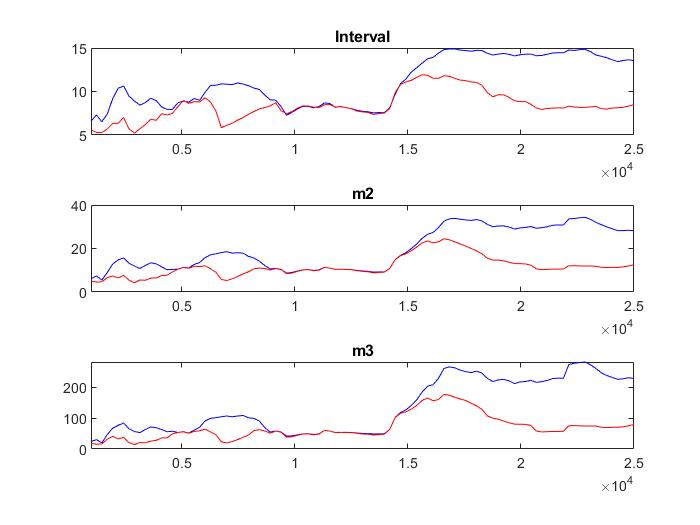
\includegraphics[scale=0.5]{mcmctay.jpg}
\label{mcmctay}
\end{figure}

\begin{figure}
    \centering 
    \begin{minipage}[t]{8.2cm} 
        \centering 
        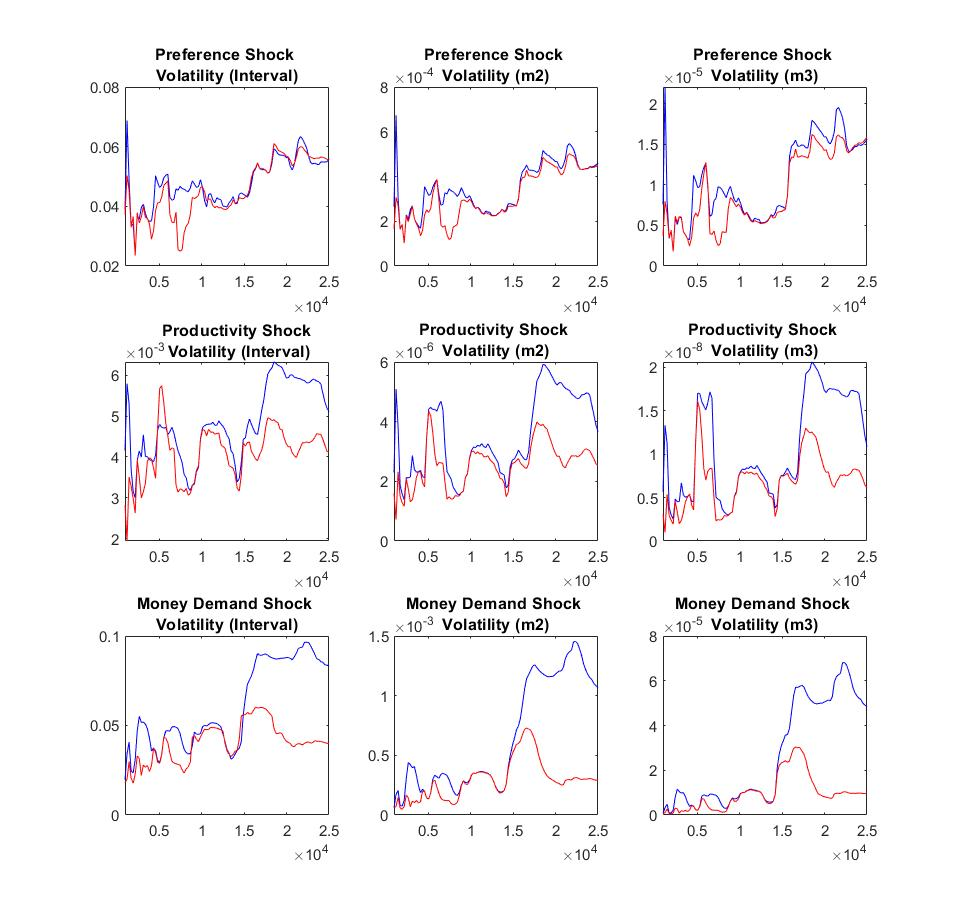
\includegraphics[width=\linewidth]{mctay1.jpg} 
    \end{minipage} 
    \hspace{0.1cm} 
    \begin{minipage}[t]{8.2cm} 
        \centering 
        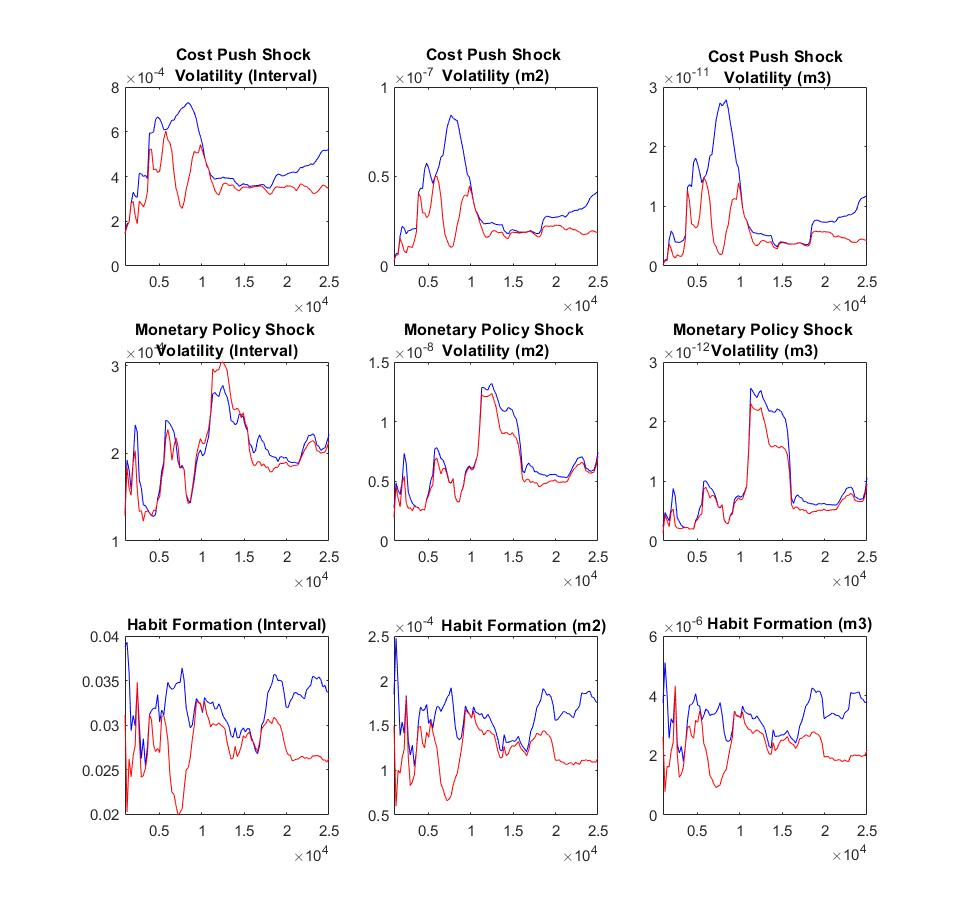
\includegraphics[width=\linewidth]{mctay2.jpg} 
    \end{minipage}
    \caption{(a) MCMC - Taylor Rule}
    \label{mctay12}
\end{figure}

\begin{figure}
    \centering 
    \begin{minipage}[t]{8.2cm} 
        \centering 
        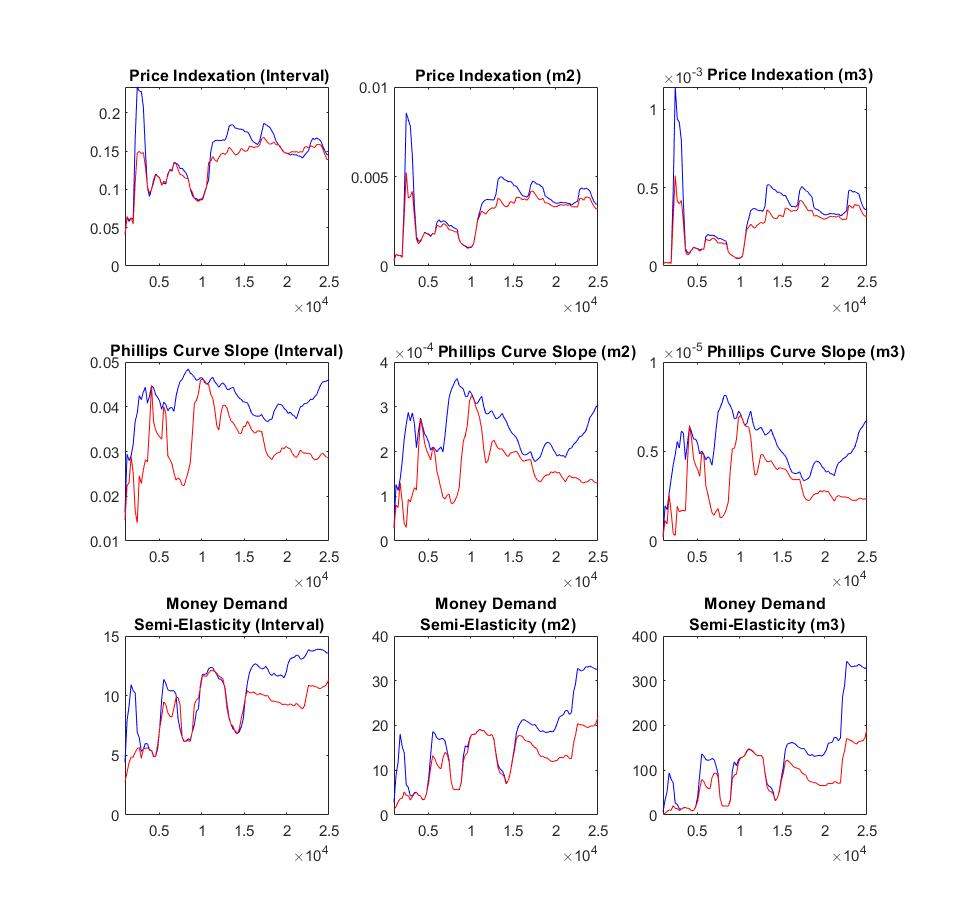
\includegraphics[width=\linewidth]{mctay3.jpg} 
    \end{minipage} 
    \hspace{0.1cm} 
    \begin{minipage}[t]{8.2cm} 
        \centering 
        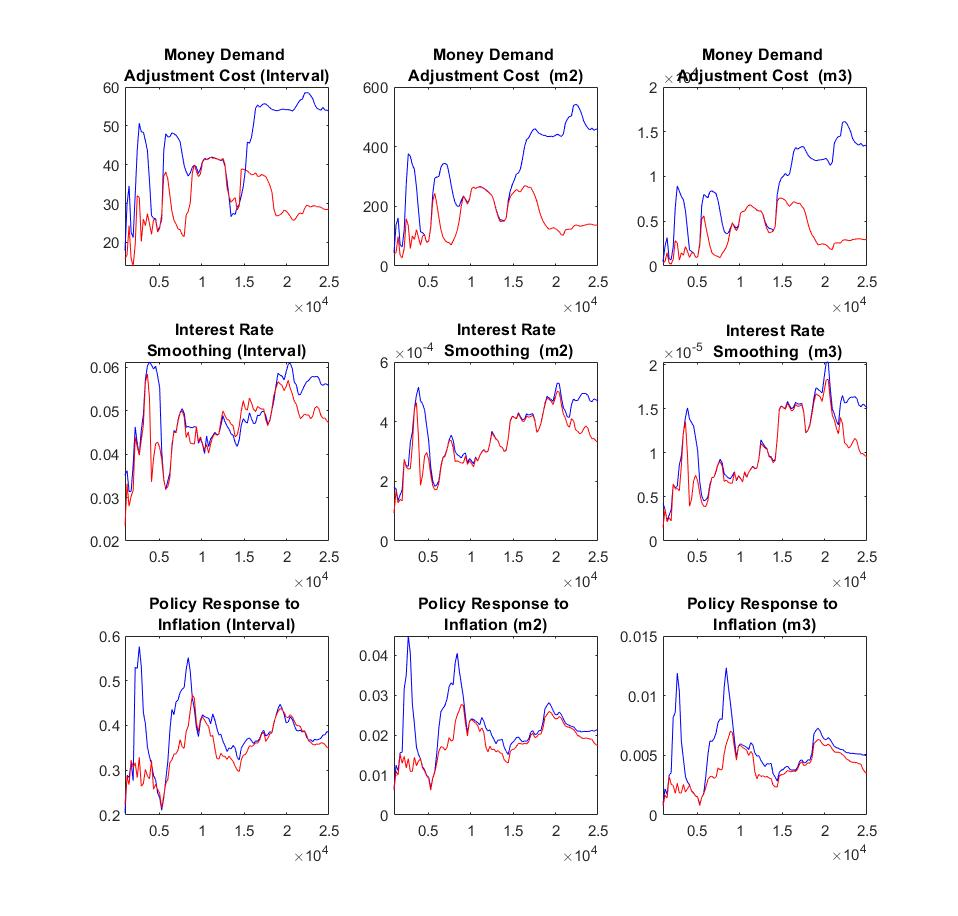
\includegraphics[width=\linewidth]{mctay4.jpg} 
    \end{minipage}
    \caption{(b) MCMC - Taylor Rule}
    \label{mctay34}
\end{figure}

\begin{figure}
    \centering 
    \begin{minipage}[t]{8.2cm} 
        \centering 
        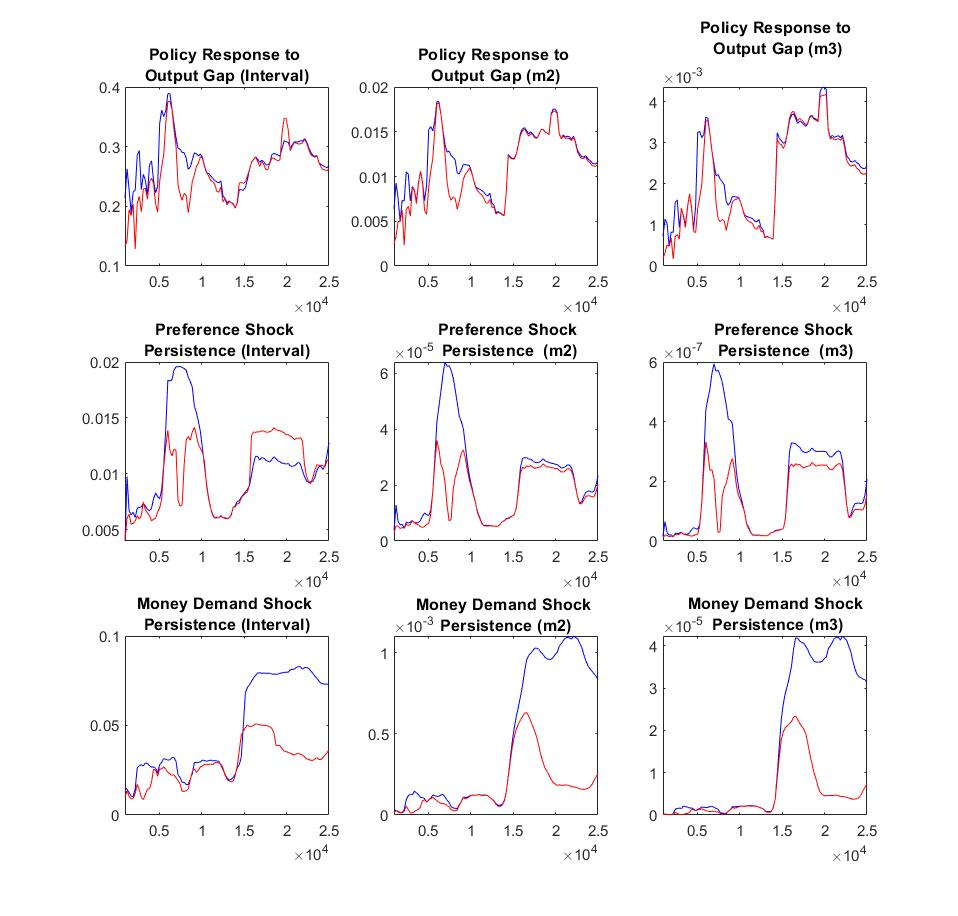
\includegraphics[width=\linewidth]{mctay5.jpg} 
    \end{minipage} 
    \hspace{0.1cm} 
    \begin{minipage}[t]{8.2cm} 
        \centering 
        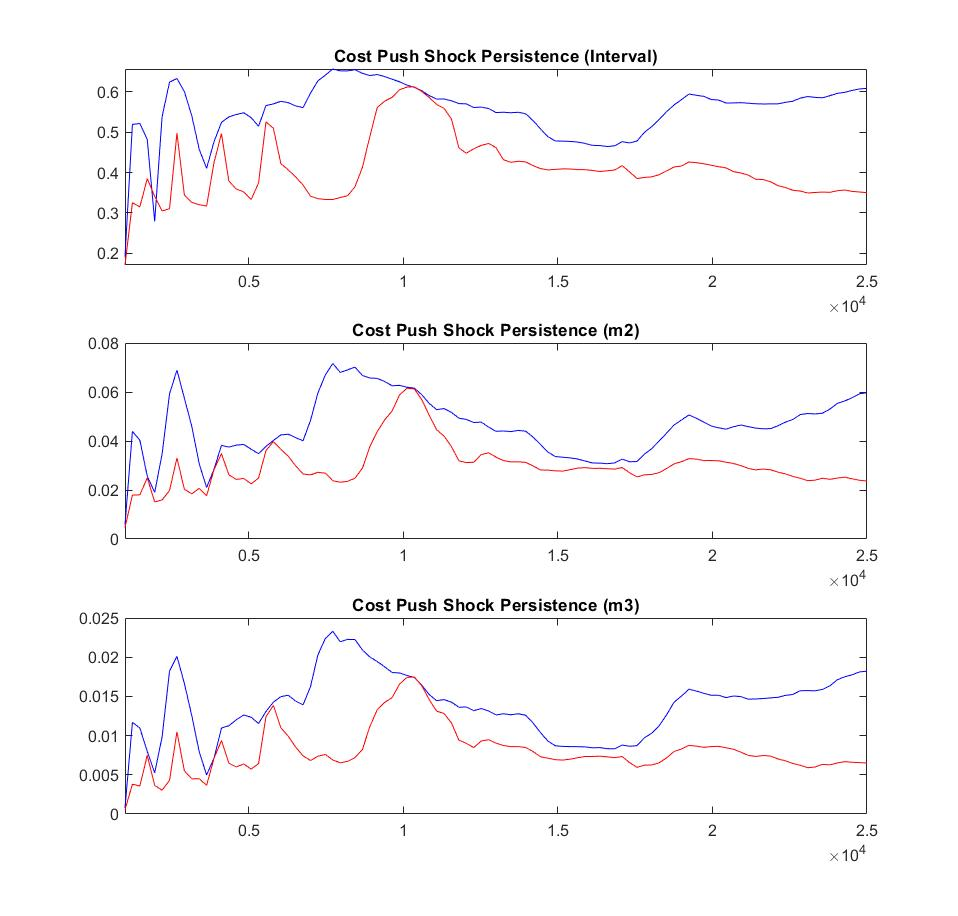
\includegraphics[width=\linewidth]{mctay6.jpg} 
    \end{minipage}
    \caption{(c) MCMC - Taylor Rule}
    \label{mctay56}
\end{figure}

\begin{figure}
\caption{MCMC general - Flexible Money Growth Rate Rule}
\centering
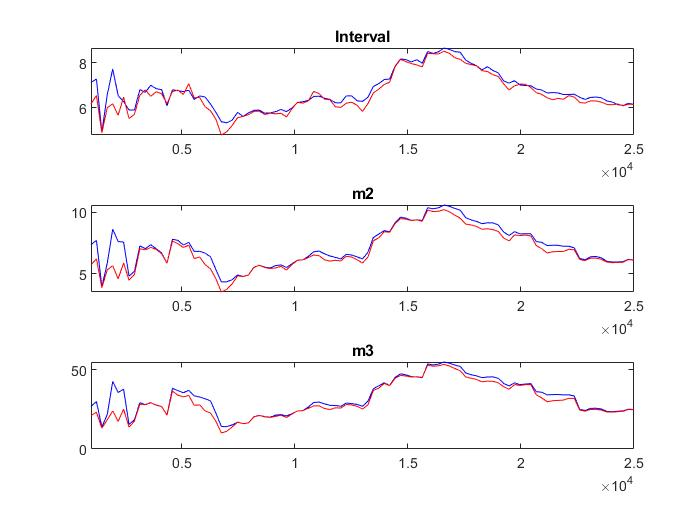
\includegraphics[scale=0.5]{mcflex.jpg}
\label{mcflex}
\end{figure}

\begin{figure}
    \centering 
    \begin{minipage}[t]{8.2cm} 
        \centering 
        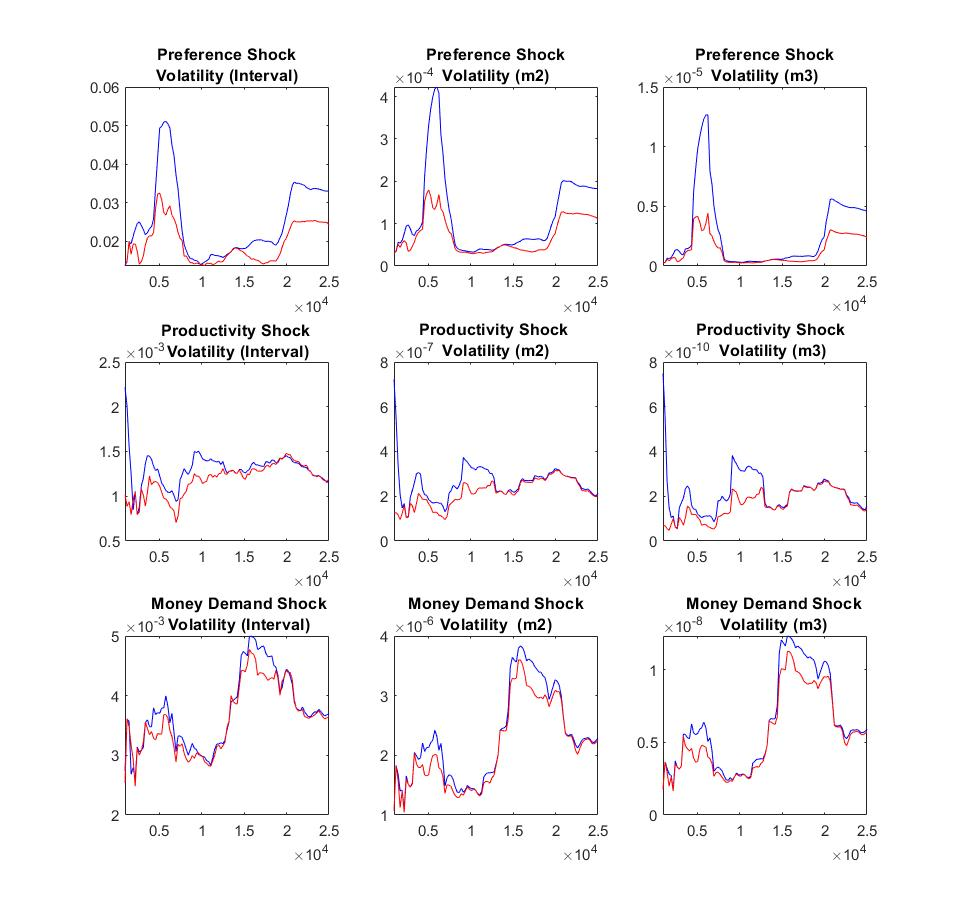
\includegraphics[width=\linewidth]{mcflex1.jpg} 
    \end{minipage} 
    \hspace{0.1cm} 
    \begin{minipage}[t]{8.2cm} 
        \centering 
        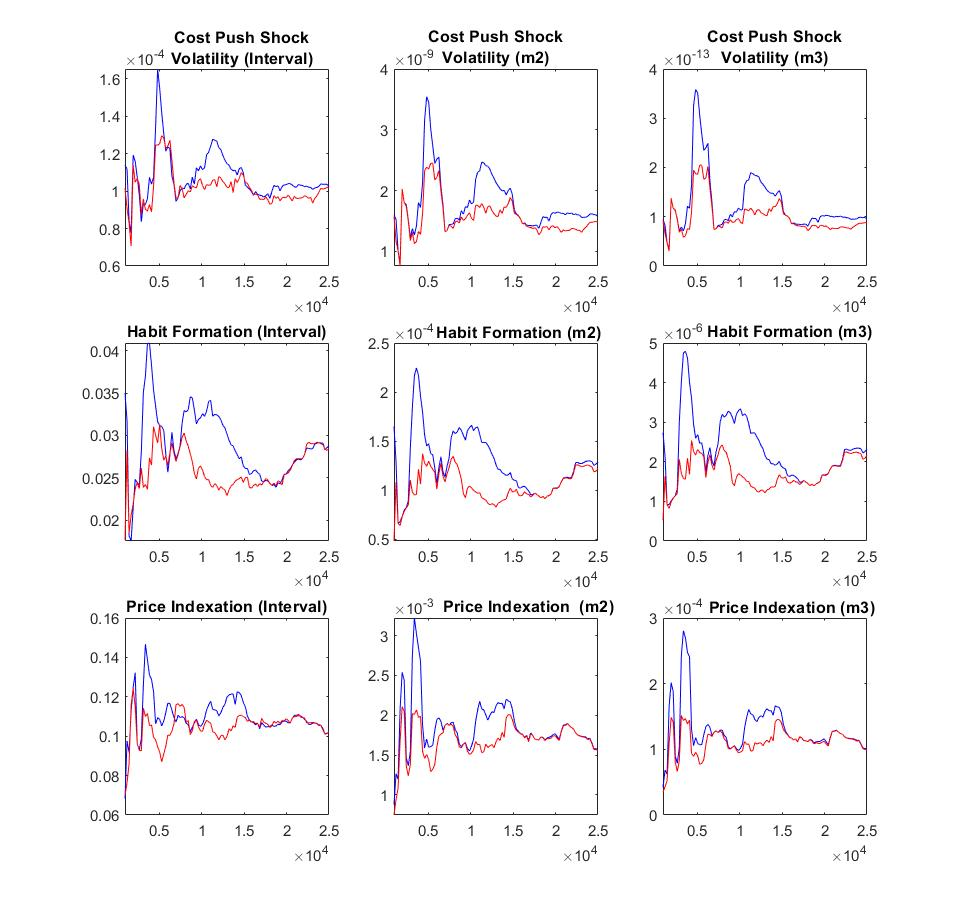
\includegraphics[width=\linewidth]{mcflex2.jpg} 
    \end{minipage}
    \caption{(a) MCMC - Flexible Money Growth Rate Rule}
    \label{mcflex12}
\end{figure}

\begin{figure}
    \centering 
    \begin{minipage}[t]{8.2cm} 
        \centering 
        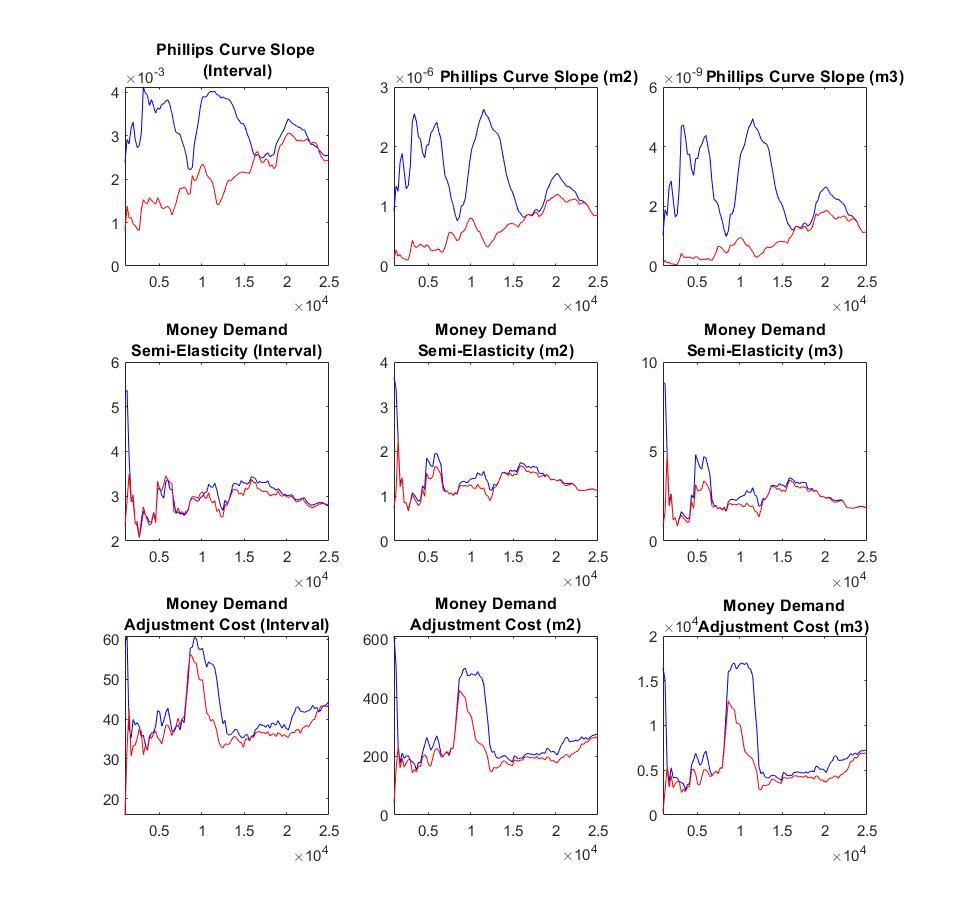
\includegraphics[width=\linewidth]{mcflex3.jpg} 
    \end{minipage} 
    \hspace{0.1cm} 
    \begin{minipage}[t]{8.2cm} 
        \centering 
        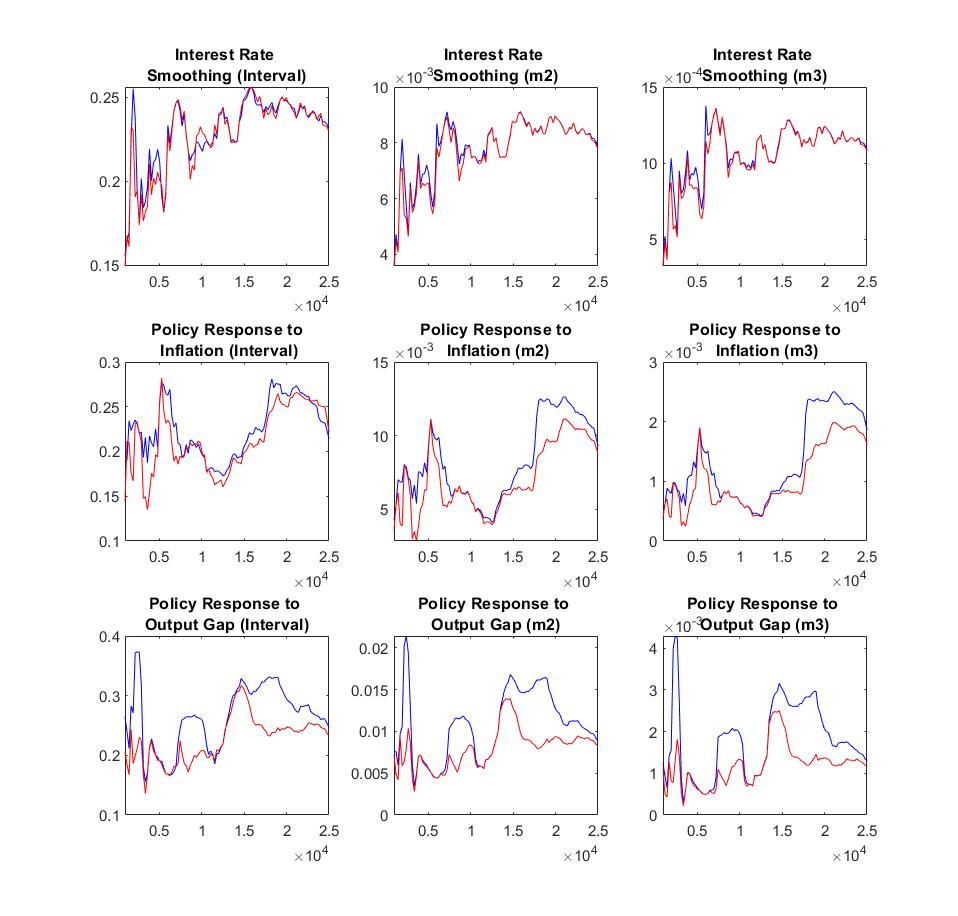
\includegraphics[width=\linewidth]{mcflex4.jpg} 
    \end{minipage}
    \caption{(b) MCMC - Flexible Money Growth Rate Rule}
    \label{mcflex34}
\end{figure}

\begin{figure}
\centering
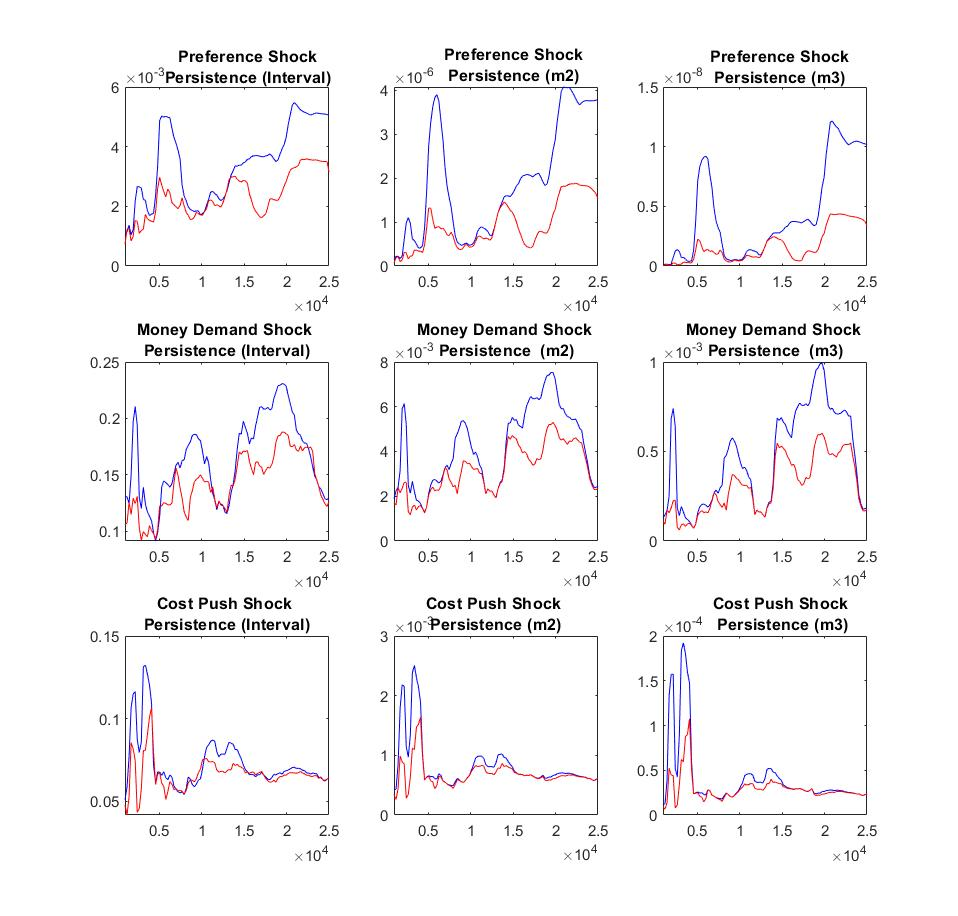
\includegraphics[scale=0.3]{mcflex5.jpg}
\caption{(c) MCMC general - Flexible Money Growth Rate Rule}
\label{mcflex5}
\end{figure}

\begin{figure}
\caption{MCMC general - Constant Money Growth Rule}
\centering
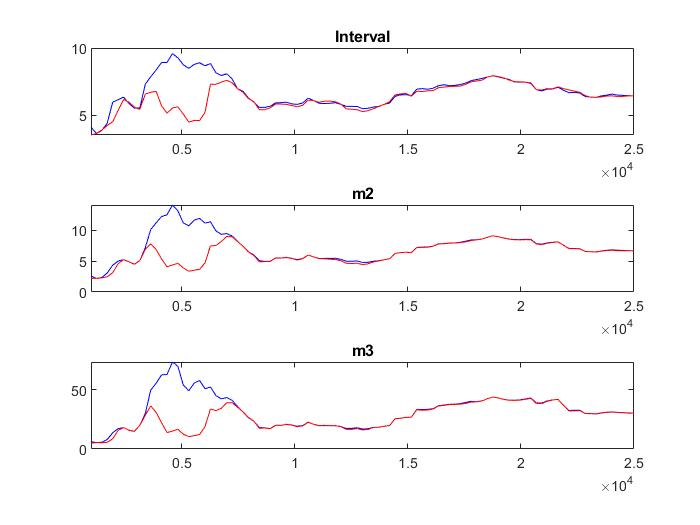
\includegraphics[scale=0.5]{mccon.jpg}
\label{mccon}
\end{figure}

\hypertarget{prior-posterior-plot}{%
\subsection{Prior-Posterior Plot}\label{prior-posterior-plot}}

Understanding the impact that the prior distribution has on the
posterior density is very important. The impact of the priors is is
extremely important to the model complexity and the structure of the
data. Figure \ref{tay_pp} and figure \ref{flex_pp} display the
relationship between the prior and the posterior. The gray line shows
the prior distribution that is also displayed in figure \ref{fig:prior1}
and figure \ref{fig:prior2}. The black line shows the density of the
posterior distribution and the green line shows the posterior mode.
Figure \ref{tay_pp} shows the prior and posterior plots for the Taylor
rule. All the plots prior and posterior distributions are vastly
different, except for money demand semi-elasticity (\(\delta_r\)) and
policy response to output gap (\(\rho_x\)). This can be due to the fact
the prior is an very accurate reflection of the information in the data.
However, more likely, it is due to that fact that (\(\rho_x\)) and
(\(\delta_r\)) are only weakly identified and that the data proves
limited information to update the prior.

Figure \ref{flex_pp} displays the prior and posterior plots for the
flexible money growth rule. The prior and posterior distributions of
interest rate smoothing (\(\rho_r\)), policy response to inflation
(\(\rho_\pi\)) and policy response to output gap (\(\rho_x\)) are
extremely similar. This is of concern as it is an indication that the
parameters were only weakly identified.

\begin{figure}
    \centering 
    \begin{minipage}[t]{8.2cm} 
        \centering 
        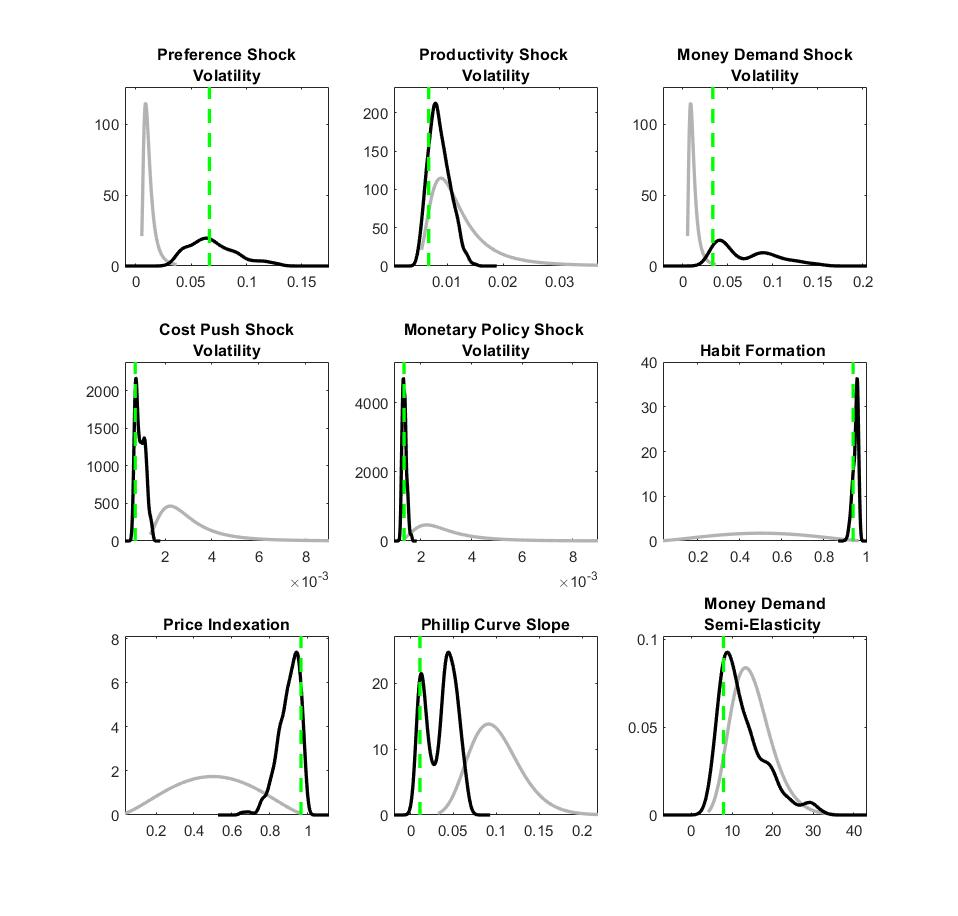
\includegraphics[width=\linewidth]{tay_pp1.jpg} 
    \end{minipage} 
    \hspace{0.1cm} 
    \begin{minipage}[t]{8.2cm} 
        \centering 
        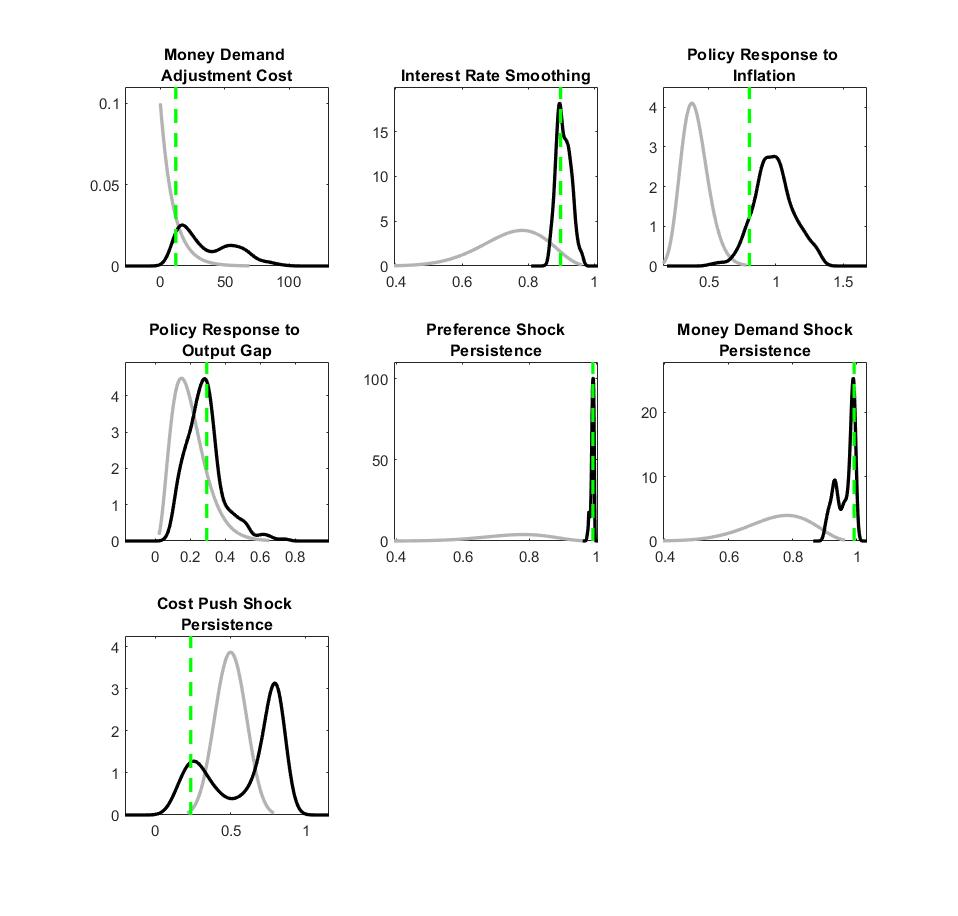
\includegraphics[width=\linewidth]{tay_pp2.jpg} 
    \end{minipage}
    \caption{Priors and Posterior: Taylor Rule}
    \label{tay_pp}
\end{figure}

\begin{figure}
    \centering 
    \begin{minipage}[t]{8.2cm} 
        \centering 
        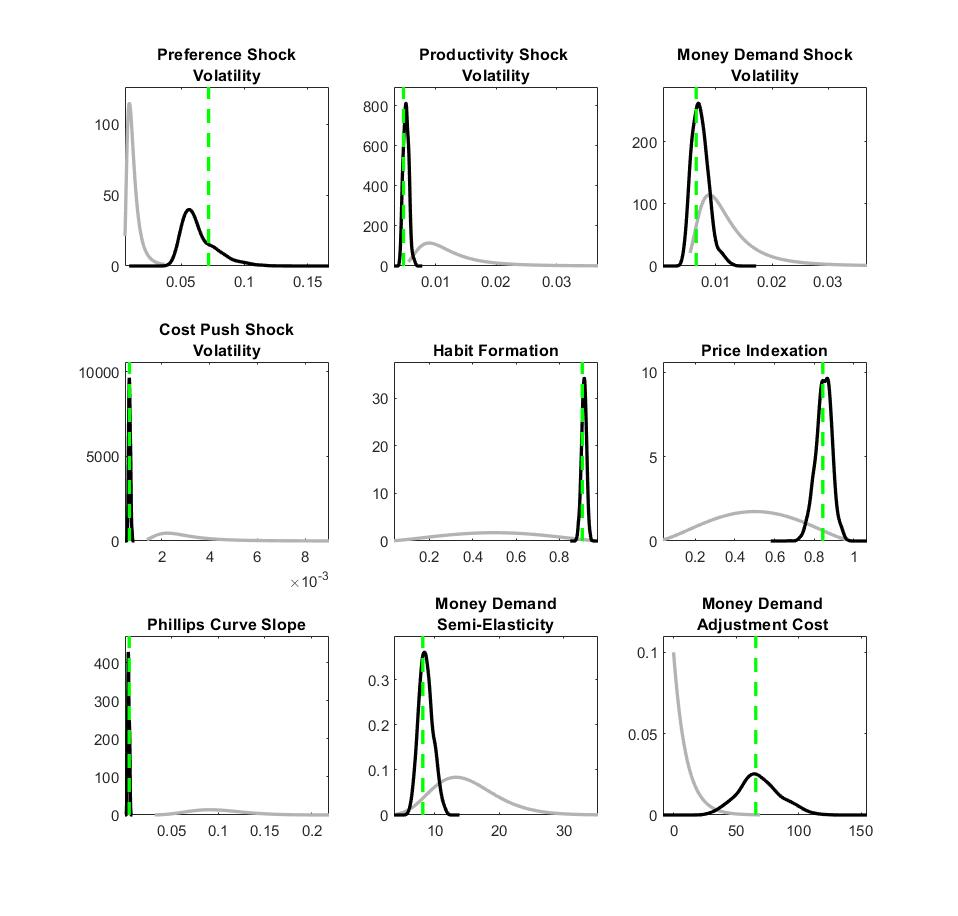
\includegraphics[width=\linewidth]{flex_pp1.jpg} 
    \end{minipage} 
    \hspace{0.1cm} 
    \begin{minipage}[t]{8.2cm} 
        \centering 
        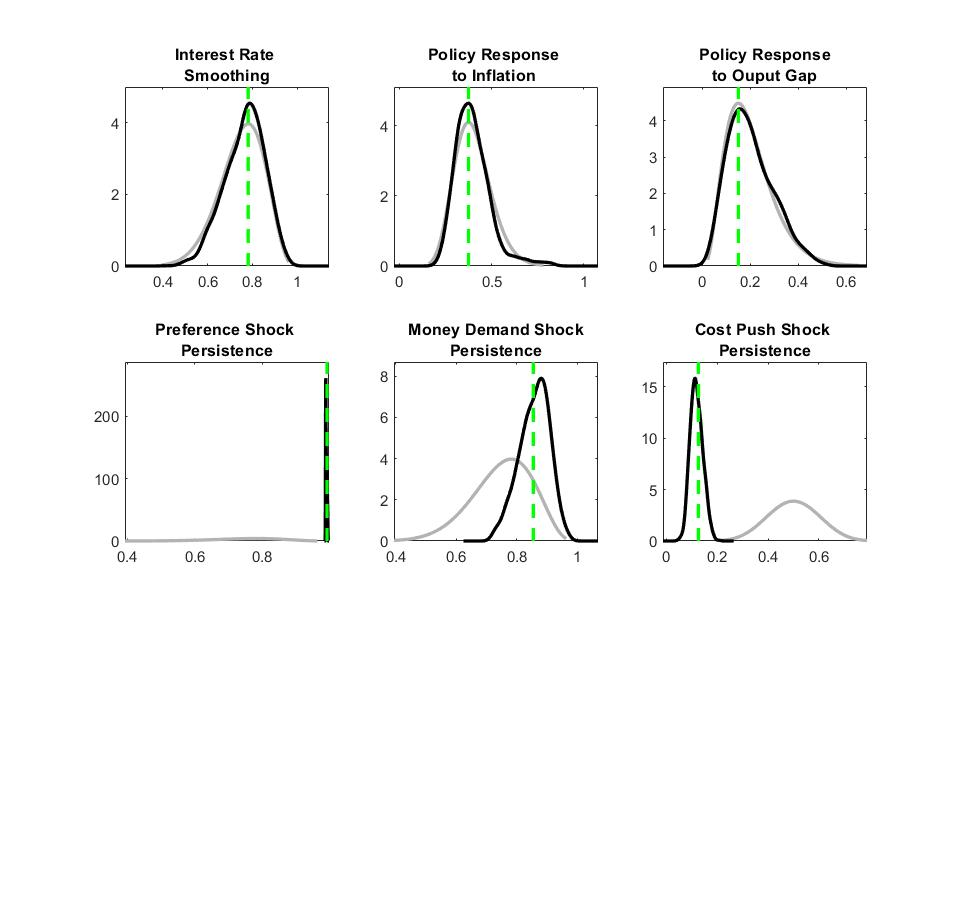
\includegraphics[width=\linewidth]{flex_pp2.jpg} 
    \end{minipage}
    \caption{Prior and Posterior: Flexible Money Growth Rule}
    \label{flex_pp}
\end{figure}

\hypertarget{smoothed-shocks}{%
\subsection{Smoothed Shocks}\label{smoothed-shocks}}

Smoothed shocks are a reconstructions of the best estimate of the values
of the unobserved shocks over the entire sample period, using the
observed data. Figure \ref{smooth} show that the structural shocks to
both the Taylor rule and the flexible money growth rule are stationary
around a mean of zero (the red line).

Figure \ref{smooth} shows a significant shock at around 75 periods for
preference and productivity shock for both rules. This volatility
represents the 2001 recession, where a decline in economic activity was
short lived and occurred mainly in developed countries. Further
volatility can be seen around 110 periods for money demand shock, cost
push shock and preference shock, representing the 2007/2008 financial
crisis. The monetary policy shock in the Taylor rule seems to be
relatively stable. Preference shocks seem to be more volatile under the
flexible money growth rule. However, the general results remain that the
flexible money growth rule and Taylor rule estimate similar volatility
of the respective shocks.

\begin{figure}
    \centering 
    \begin{minipage}[t]{8.2cm} 
        \centering 
        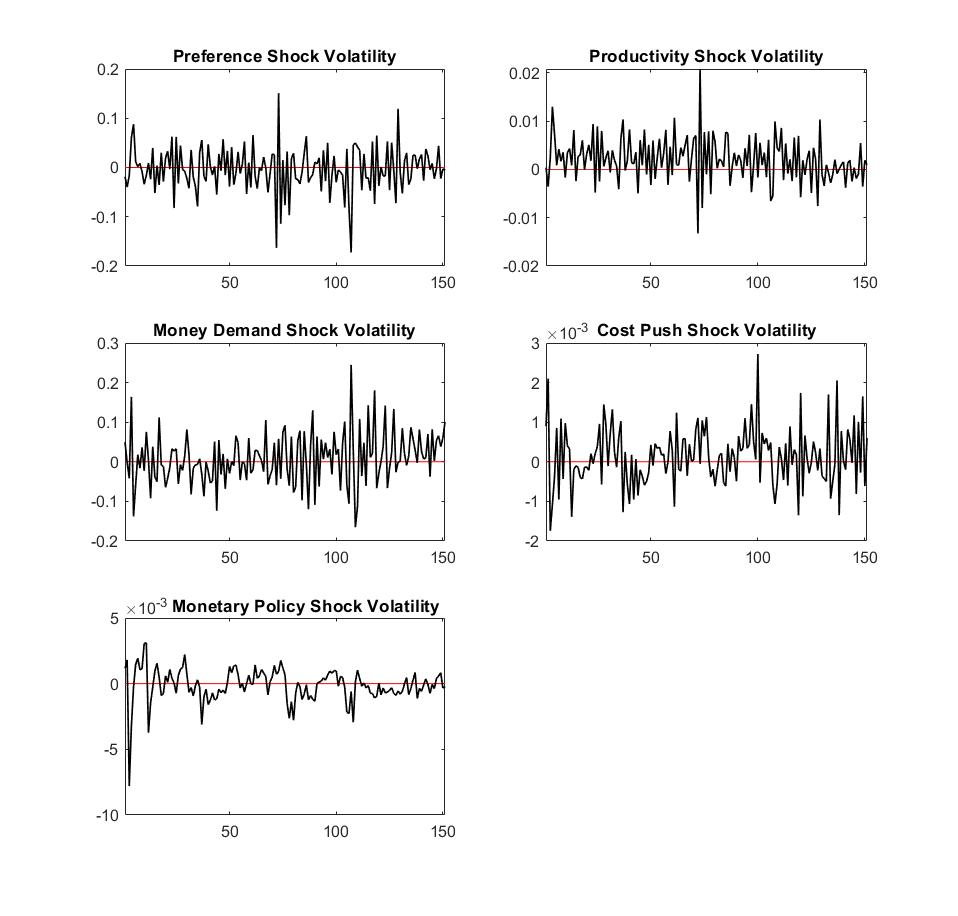
\includegraphics[width=\linewidth]{tay_smooth.jpg} 
        \caption{Taylor Rule}
    \end{minipage} 
    \hspace{0.1cm} 
    \begin{minipage}[t]{8.2cm} 
        \centering 
        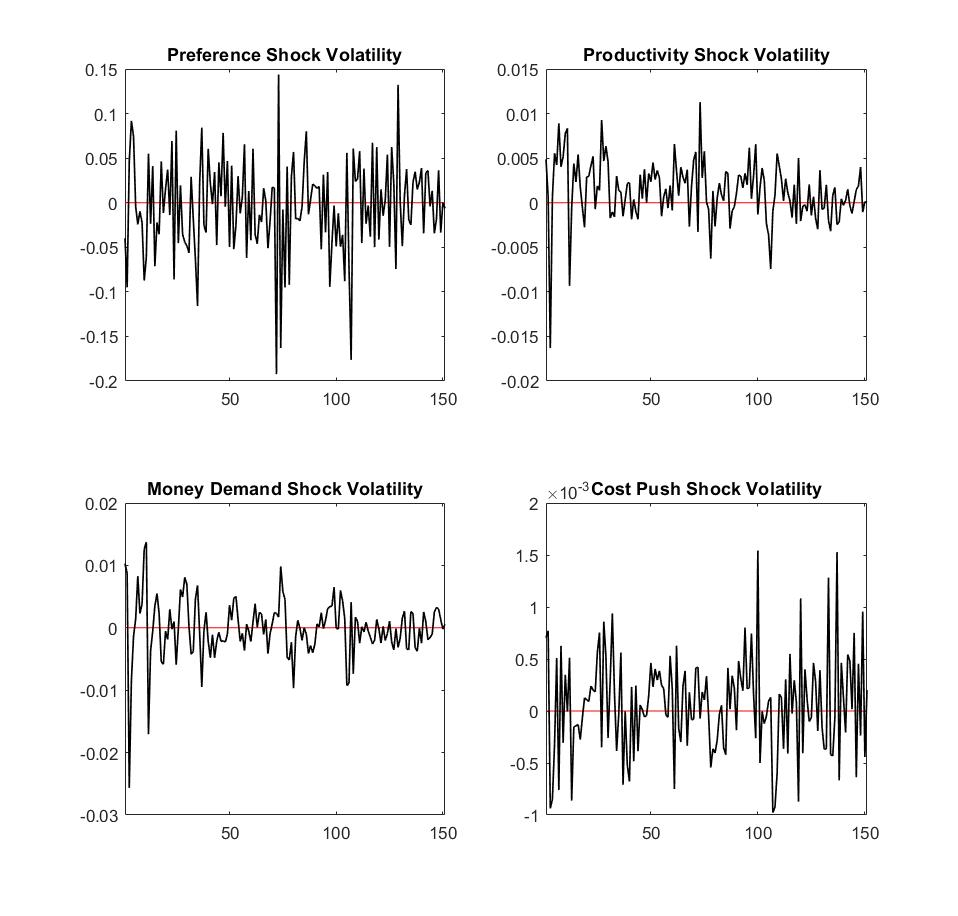
\includegraphics[width=\linewidth]{flex_smooth.jpg} 
        \caption{Flexible Monetary Policy Rule}
    \end{minipage}
    \caption{Smoothed shocks}
    \label{smooth}
\end{figure}

\hypertarget{historical-and-smooth-variables}{%
\subsection{Historical and Smooth
Variables}\label{historical-and-smooth-variables}}

Figure \ref{hs} represent historical and smoothed variable plots. The
analysis is done is order to determine whether measurement error exist
in our model. The dotted black line represents the actual data that is
observed and the red line represents the estimate of the smoothed
variable. Under the Taylor rule and flexible money growth rate rule both
series are identical as they overlap eachother, implying that there is
no measurement error and that model is specified correctly. This is
another indication that the flexible money growth rate rule preforms
just as well as the Taylor rule.

\begin{figure}
    \centering 
    \begin{minipage}[t]{8.2cm} 
        \centering 
        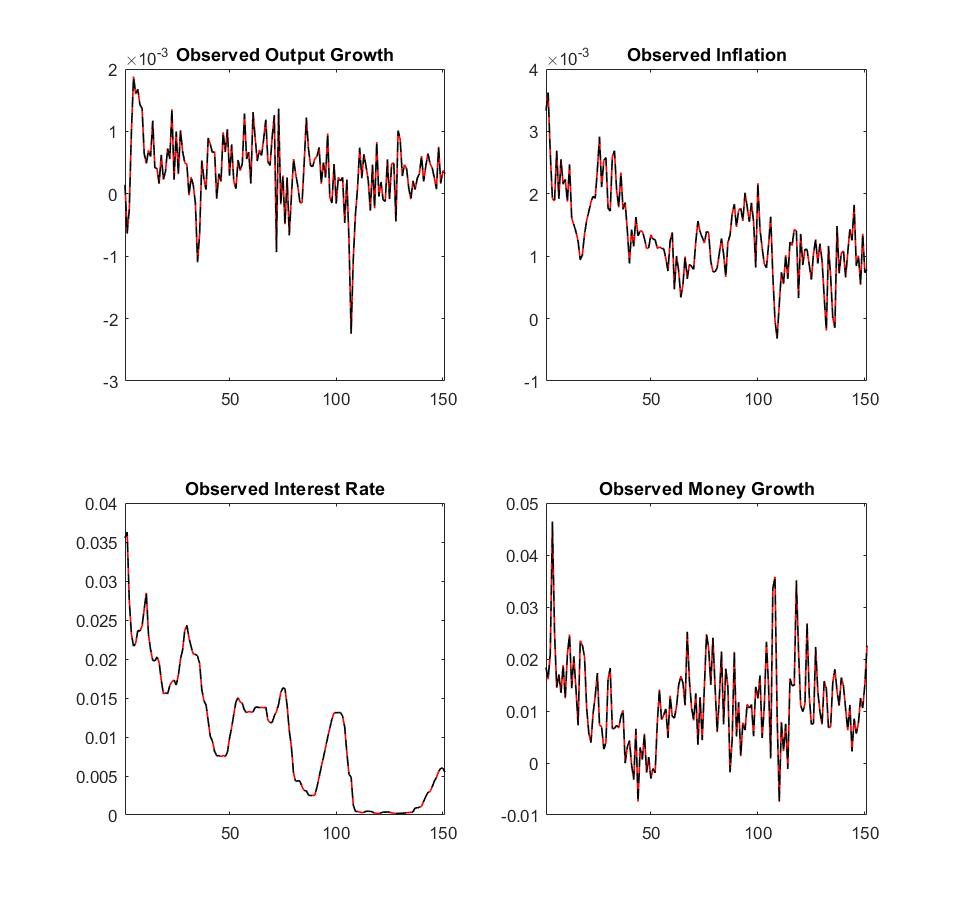
\includegraphics[width=\linewidth]{tay_hs.jpg} 
        \caption{Taylor Rule}
    \end{minipage} 
    \hspace{0.1cm} 
    \begin{minipage}[t]{8.2cm} 
        \centering 
        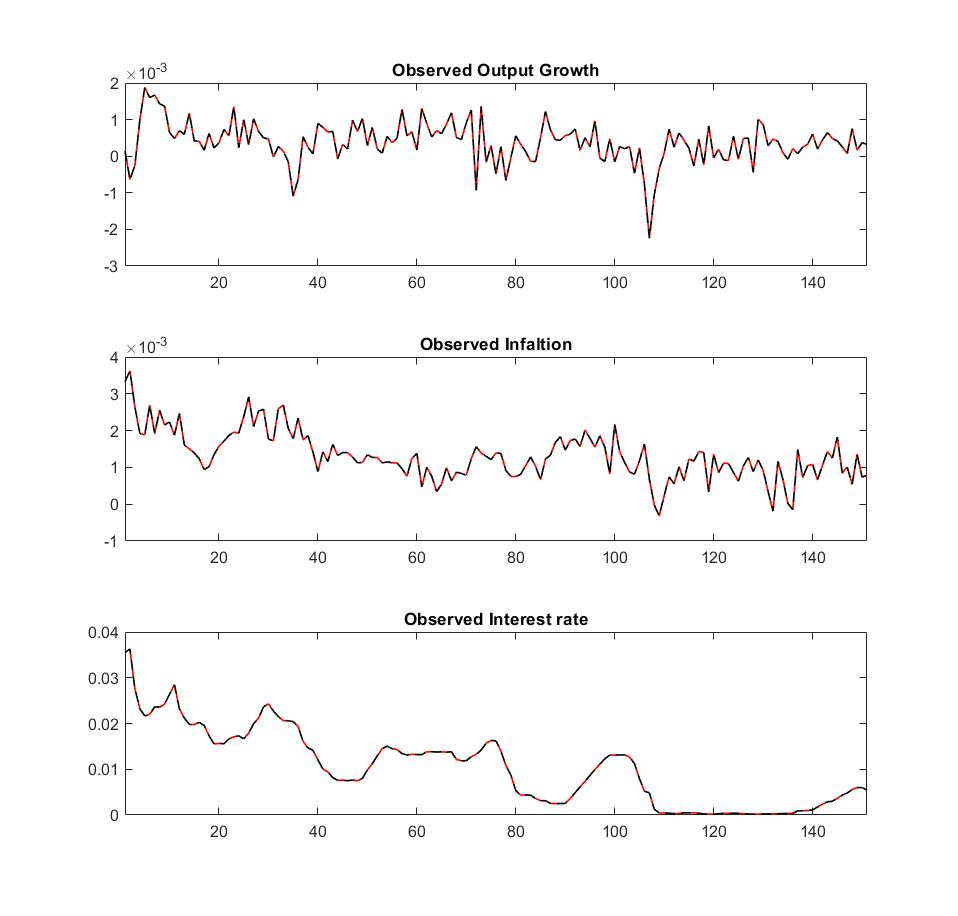
\includegraphics[width=\linewidth]{flex_hs.jpg} 
        \caption{Flexible Monetary Policy Rule}
    \end{minipage}
    \caption{Historical and Smooth Variables}
    \label{hs}
\end{figure}

\hypertarget{variance-decomposition}{%
\subsection{Variance Decomposition}\label{variance-decomposition}}

The variance decomposition displayed in table \ref{tay_var_dec} and
table \ref{flex_var_dec} is used to analyze how variation in the model
is generated by a specific shock. This method is informative in
establishing the relative importance of a specific shock as a source of
volatility to a macroeconomic variable. Productivity shocks accounts for
most of the variation in Consumption (\(c\)), output (\(\hat{y}\)) and
the efficient level of output (\(\hat{q}\)) under the Taylor rule and
the flexible money growth rule. Whereas a cost push shock accounts for
most of the variation in inflation (\(\pi\)). Variation in monetary
policy shock (\(r\)) is explained mostly by preference shock {[}60.86
percent and 51.09 percent{]}, with cost push shock also explaining a
large portion of the variation in the Taylor rule and flexible money
growth rule, respectively.

Under the Taylor rule, variation in money growth (\(\mu\)) and money
demand (\(\hat{m}\)) is largely explained by a monetary demand shock.
However, under the flexible money growth rule, money demand
(\(\hat{m}\)) is mostly explained by a preference shock and money growth
(\(\mu\)) is explained by similar by a preference shock, productivity
shock and cost push shock.

\begin{table}
\caption{Taylor Rule: Posterior Mean Variance Decomposition (in percent)}
 \begin{center}
\begin{tabular}{|c|c|c|c|c|c|c|}
\hline
  & Description &   ${\sigma_a}$  &  ${\sigma_z}$ & ${\sigma_u}$ & ${\sigma_e}$ & ${\sigma_r}$\\
\hline
${c}$ & consumption & 82.04 & 17.81 & 0.00 & 0.14 & 0.00 \\
 ${\hat y}$  & output & 82.04 & 17.81 & 0.00 & 0.14 & 0.00 \\
 ${\lambda}$ & lambda & 99.38 & 0.00 & 0.00 & 0.60 & 0.02 \\
${a}$ & preference shock & 100.00 & 0.00 & 0.00 & 0.00 & 0.00 \\
${z}$ & productivity shock & 0.00 & 100.00 & 0.00 & 0.00 & 0.00 \\
 ${r}$ & monetary policy shock & 60.86 & 0.00 & 0.00 & 30.33 & 8.80 \\
${\pi}$ & inflation & 17.85 & 0.00 & 0.00 & 72.23 & 9.91 \\
${\hat q}$ & efficient level of output & 82.13 & 17.87 & 0.00 & 0.00 & 0.00 \\
 ${x}$ & output gap & 0.99 & 0.00 & 0.00 & 98.21 & 0.80 \\
${e}$ & cost push shock & 0.00 & 0.00 & 0.00 & 100.00 & 0.00 \\
${u}$ & money demand shock & 0.00 & 0.00 & 100.00 & 0.00 & 0.00 \\
${\hat m}$ & money demand & 9.69 & 0.51 & 87.62 & 3.99 & 1.31\\
${\mu}$  & money growth & 1.83 & 3.25 & 89.62 & 3.99 & 1.31 \\
${\hat g}$ & output growth & 49.20 & 49.00 & 0.00 & 1.75 & 0.05\\
\hline
\end{tabular}
\end{center}
\label{tay_var_dec}
\end{table}

\begin{table}
\caption{Flexible Monetary Policy Rule: Posterior Mean Variance Decomposition (in percent)}
 \begin{center}
\begin{tabular}{|c|c|c|c|c|c|}
\hline
  & Description &   ${\sigma_a}$  &  ${\sigma_z}$ & ${\sigma_u}$ & ${\sigma_e}$ \\ 
\hline
${c}$ & consumption & 89.54 & 10.36 & 0.02 & 0.08 \\
 ${\hat y}$  & output & 89.54 & 10.36 & 0.02 & 0.08 \\
 ${\lambda}$ & lambda & 99.87 & 0.06& 0.02 & 0.05 \\
${a}$ & preference shock & 100.00 & 0.00 & 0.00 & 0.00 \\
${z}$ & productivity shock & 0.00 & 100.00 & 0.00 & 0.00 \\
 ${r}$ & monetary policy shock & 51.09 & 12.88 & 9.23 & 26.80 \\
${\pi}$ & inflation & 6.73 & 7.69 & 1.31 & 84.27 \\
${\hat q}$ & efficient level of output & 90.64 & 9.36 & 0.00 & 0.00 \\
 ${x}$ & output gap & 27.43 & 32.38 & 6.40 & 33.79 \\
${e}$ & cost push shock & 0.00 & 0.00 & 0.00 & 100.00 \\
${u}$ & money demand shock & 0.00 & 0.00 & 100.00 & 0.00 \\
${\hat m}$ & money demand & 74.40 & 17.01 & 1.52 & 7.08 \\
${\mu}$  & money growth & 25.09 & 33.15 & 3.44 & 38.33 \\
${\hat g}$ & output growth & 52.27 & 44.91 & 0.68 & 2.13 \\
\hline
\end{tabular}
\end{center}
\label{flex_var_dec}
\end{table}

\hypertarget{forecasting}{%
\subsection{Forecasting}\label{forecasting}}

Figure \ref{tay_mean} and figure \ref{flex_mean} displays the mean
forecast plots of the Taylor rule and flexible money growth rule,
respectively. The black line represents the mean forecasts of the
macroeconomic endogenous variable, starting at the last observation in
the sample and going 40 periods ahead. The green lines represent the
mean forecast deciles. It is important to note that the forecasts only
take parameter uncertainty into account and not the uncertainty about
future shocks. Under the flexible money growth rule, the macroeconomic
variable appear to stabilize to their steady state faster than the under
the Taylor rule. This, once again, established that the flexible money
growth rule could be more optimal than the Taylor rule.

\begin{figure}
    \centering 
    \begin{minipage}[t]{8.2cm} 
        \centering 
        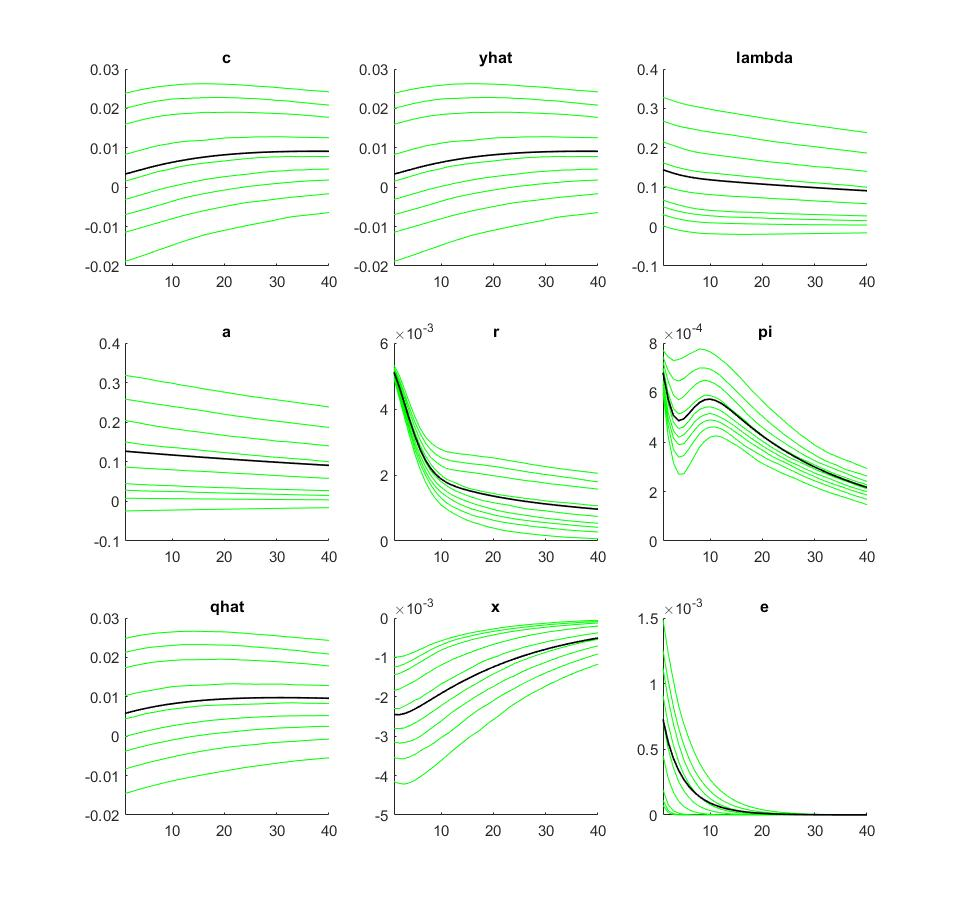
\includegraphics[width=\linewidth]{tay_fore_mean.jpg} 
    \end{minipage} 
    \hspace{0.1cm} 
    \begin{minipage}[t]{8.2cm} 
        \centering 
        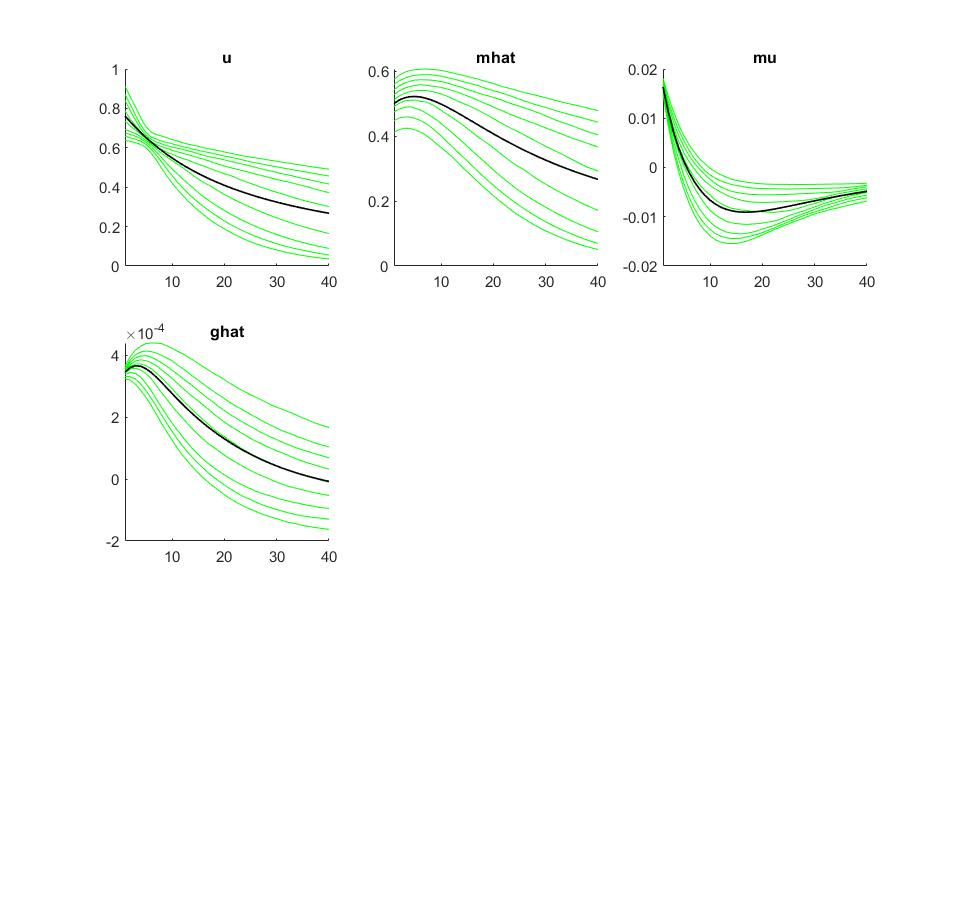
\includegraphics[width=\linewidth]{tay_fore_mean1.jpg} 
    \end{minipage}
    \caption{Forecasted Variables (mean) - Taylor Rule}
    \label{tay_mean}
\end{figure}

\begin{figure}
    \centering 
    \begin{minipage}[t]{8.2cm} 
        \centering 
        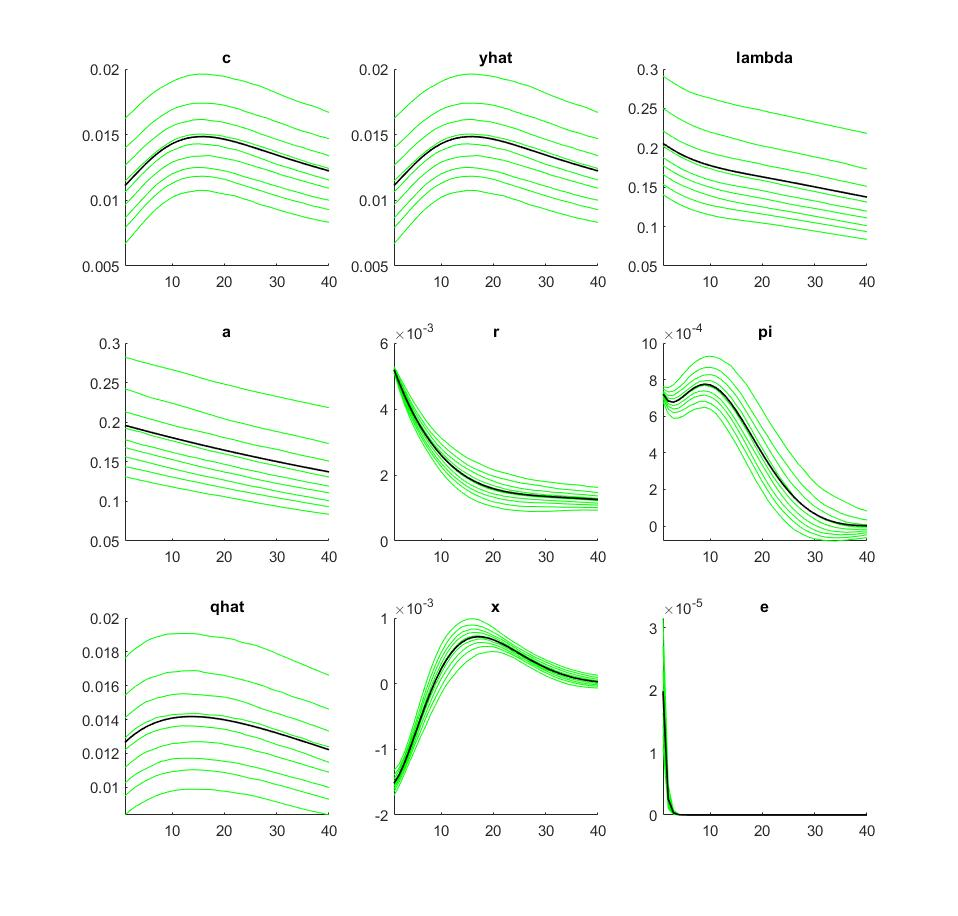
\includegraphics[width=\linewidth]{flex_fore_mean.jpg} 
    \end{minipage} 
    \hspace{0.1cm} 
    \begin{minipage}[t]{8.2cm} 
        \centering 
        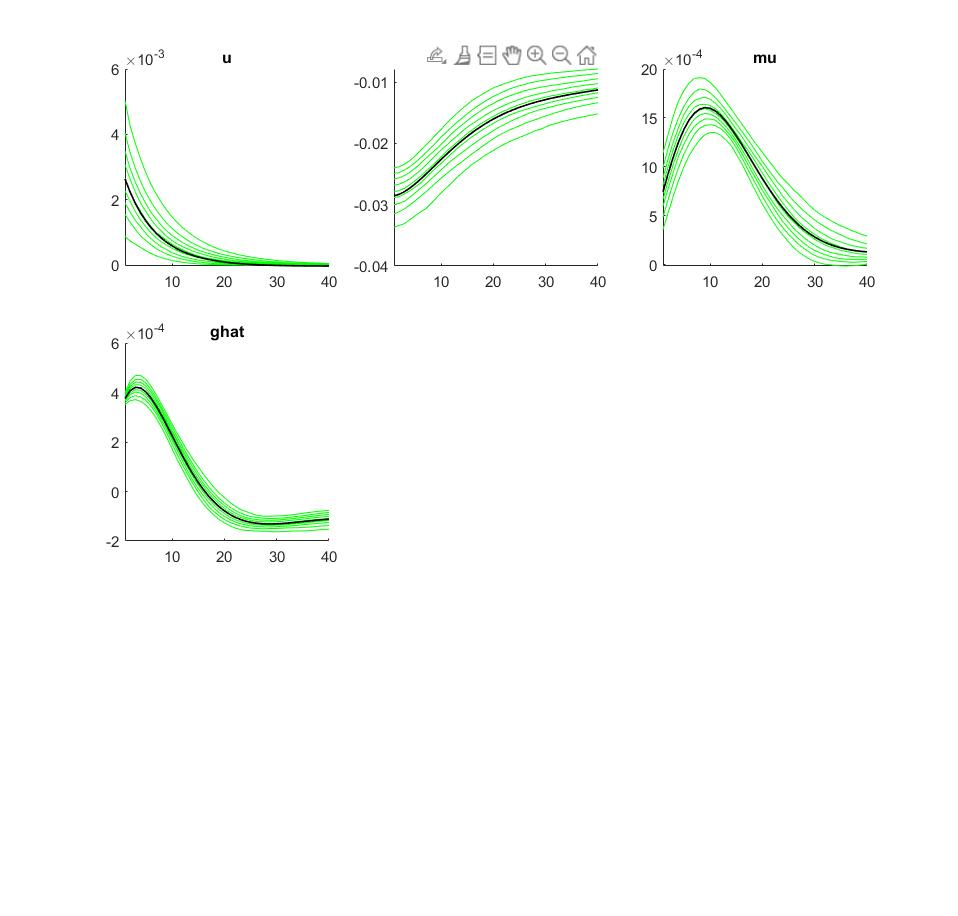
\includegraphics[width=\linewidth]{flex_fore_mean1.jpg} 
    \end{minipage}
    \caption{Forecasted Variables (mean) - Flexible Money Growth Rule}
    \label{flex_mean}
\end{figure}

Figure \ref{tay_point} and figure \ref{flex_point} displays the point
forecast plots for the Taylor rule and flexible money growth rule,
respectively. In contrast to the mean forecast, the point forecast takes
the parameter uncertainty and the uncertainty about future shocks into
account. Both rules have very similar results, with the exception being
the output gap (\(x\)) and the money demand shock (\(u\)), which both
appear to stabilize around the steady state faster under the flexible
money growth rule.

\begin{figure}
    \centering 
    \begin{minipage}[t]{8.2cm} 
        \centering 
        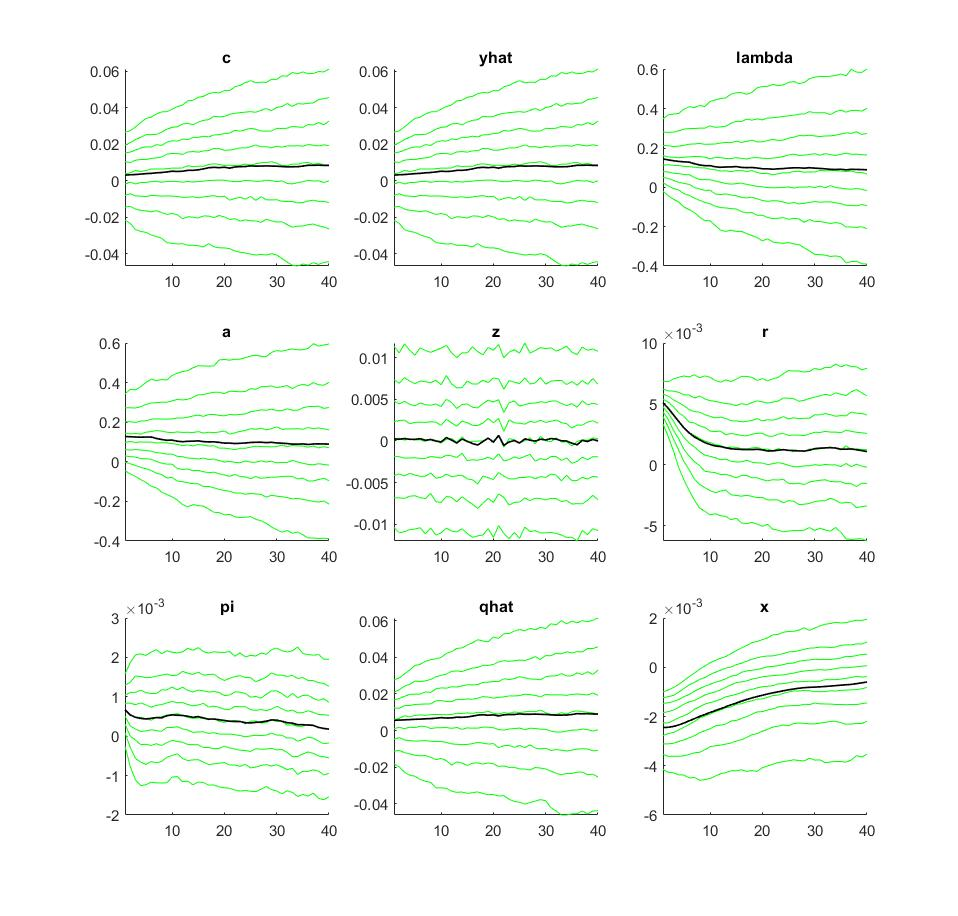
\includegraphics[width=\linewidth]{tay_fore_var1.jpg} 
    \end{minipage} 
    \hspace{0.1cm} 
    \begin{minipage}[t]{8.2cm} 
        \centering 
        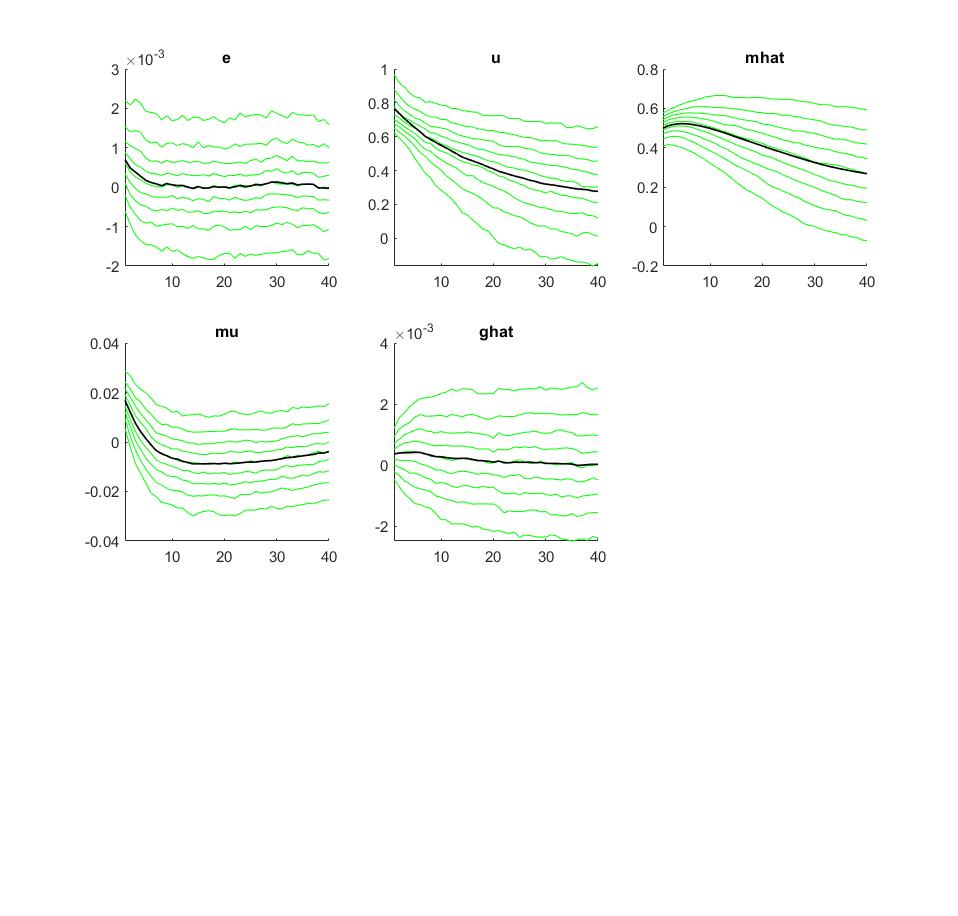
\includegraphics[width=\linewidth]{tay_fore_var2.jpg} 
    \end{minipage}
    \caption{Forecasted Variables (point) - Taylor Rule}
    \label{tay_point}
\end{figure}

\begin{figure}
    \centering 
    \begin{minipage}[t]{8.2cm} 
        \centering 
        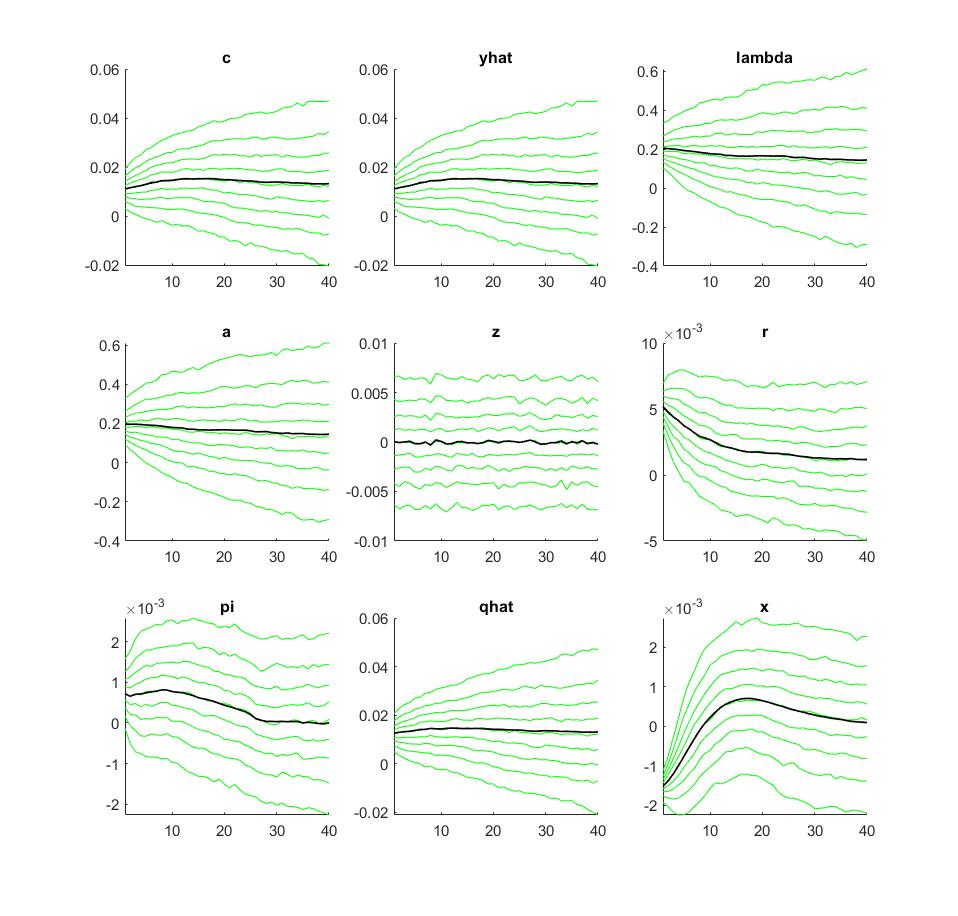
\includegraphics[width=\linewidth]{flex_fore_var1.jpg} 
    \end{minipage} 
    \hspace{0.1cm} 
    \begin{minipage}[t]{8.2cm} 
        \centering 
        \includegraphics[width=\linewidth]{flex_fore_var2.jpg} 
    \end{minipage}
    \caption{Forecasted Variables (point) - Flexible Money Growth Rule}
    \label{flex_point}
\end{figure}

\hypertarget{conclusion}{%
\section{Conclusion}\label{conclusion}}

The central object of this project was to estimate, simulate and analyze
the effect of the Taylor rule and flexible money growth rate rule on
macroeconomic variables. Following
\protect\hyperlink{ref-belongia2019reconsideration}{Belongia, Ireland \&
others} (\protect\hyperlink{ref-belongia2019reconsideration}{2019}),
this projects makes of the DSGE model and was estimated using a Bayesian
approach. The overall findings indicate that the flexible money growth
rule comparatively similar, and in some cases better, than the Taylor
rule. This implies that policymakers should consider a flexible money
growth rate rule since it successfully decreases macroeconomic
volatility in inflation and output growth.

In the previous report, the conclusion was reach that the constant money
growth rule preformed the poorest in the simulations, therefore, only it
was only briefly mentioned. However, it remains clear that a
reconsideration of the Fed's monetary policy toolkit is warranted, and
further study along this avenue should be encouraged.

\newpage

\hypertarget{references}{%
\section*{References}\label{references}}
\addcontentsline{toc}{section}{References}

\hypertarget{refs}{}
\begin{CSLReferences}{1}{0}
\leavevmode\hypertarget{ref-bedard2008optimal}{}%
Bedard, M. 2008. Optimal acceptance rates for metropolis algorithms:
Moving beyond 0.234. \emph{Stochastic Processes and their Applications}.
118(12):2198--2222.

\leavevmode\hypertarget{ref-belongia2019reconsideration}{}%
Belongia, M.T., Ireland, P.N. \& others. 2019. \emph{A reconsideration
of money growth rules}. Boston College.

\leavevmode\hypertarget{ref-guerron2013bayesian}{}%
Guerrón-Quintana, P.A. \& Nason, J.M. 2013. Bayesian estimation of DSGE
models. In Edward Elgar Publishing \emph{Handbook of research methods
and applications in empirical macroeconomics}.

\leavevmode\hypertarget{ref-laffargue2000blanchard}{}%
Laffargue, J.-P. \& others. 2000. The blanchard and kahn's conditions in
a macroeconometric model with perfect foresight. \emph{mimeographed
Cepremap}.

\leavevmode\hypertarget{ref-smets}{}%
Smets, F. \& Wouters, R. 2007. Shocks and frictions in US business
cycles: A bayesian DSGE approach. \emph{American economic review}.
97(3):586--606.

\end{CSLReferences}

\hypertarget{appendix}{%
\section*{Appendix}\label{appendix}}
\addcontentsline{toc}{section}{Appendix}

\hypertarget{appendix-a}{%
\subsection*{Appendix A}\label{appendix-a}}
\addcontentsline{toc}{subsection}{Appendix A}

\begin{table}
\caption{Endogenous Variables}
 \label{Table:end}
 \begin{center}
\begin{tabular}{|c|c|c|} 
\hline
  Variable & Symbol & Description \\ 
\hline
\texttt{c} & ${c}$ & consumption\\
\texttt{yhat} & ${\hat y}$ & output\\
\texttt{lambda} & ${\lambda}$ & lambda\\
\texttt{a} & ${a}$ & preference shock\\
\texttt{z} & ${z}$ & productivity shock\\
\texttt{r} & ${r}$ & monetary policy shock\\
\texttt{pi} & ${\pi}$ & inflation\\
\texttt{qhat} & ${\hat q}$ & efficient level of output\\
\texttt{x} & ${x}$ & output gap\\
\texttt{e} & ${e}$ & cost push shock\\
\texttt{u} & ${u}$ & money demand shock\\
\texttt{mhat} & ${\hat m}$ & money demand\\
\texttt{mu} & ${\mu}$ & money growth\\
\texttt{ghat} & ${\hat g}$ & output growth\\
\texttt{gobs} & ${g^{obs}}$ & observed output growth\\
\texttt{piobs} & ${\pi^{obs}}$ & observed inflation\\
\texttt{robs} & ${r^{obs}}$ & observed interest rate\\
\texttt{muobs} & ${\mu^{obs}}$ & observed money growth\\
\hline
\end{tabular}
\end{center}
\end{table}

\begin{table}
\caption{Parameters}
 \label{Table:para}
 \begin{center}
\begin{tabular}{|c|c|c|} 
\hline
  Variable & Symbol & Description \\ 
\hline
\texttt{z\_ss} & ${z_{ss}}$ & output growth steady state\\
\texttt{beta} & ${\beta}$ & discount factor\\
\texttt{gamma} & ${\gamma}$ & habit formation\\
\texttt{rho\_a} & ${\rho_a}$ & preference shock persistence\\
\texttt{alpha} & ${\alpha}$ & price indexation\\
\texttt{psi} & ${\psi}$ & Phillips curve slope\\
\texttt{rho\_r} & ${\rho_r}$ & interest rate smoothing\\
\texttt{rho\_pi} & ${\rho_\pi}$ & policy response to inflation\\
\texttt{rho\_x} & ${\rho_x}$ & policy response to output gap\\
\texttt{delta\_r} & ${\delta_r}$ & money demand semi-elasticity \\
\texttt{phi} & ${\phi}$ & money demand adjustment cost\\
\texttt{r\_ss} & ${r_ss}$ & interest rate steady state\\
\texttt{rho\_u} & ${\rho_u}$ & money demand shock persistence\\
\texttt{rho\_e} & ${\rho_e}$ & cost push shock persistence\\
\texttt{rho\_mm} & ${\rho_mm}$ & money shock\\
\texttt{rho\_mpi} & ${\rho_m\pi}$ & money inflation shock\\
\texttt{rho\_mx} & ${\rho_mx}$ & output gap shock\\
\hline
\end{tabular}
\end{center}
\end{table}

\bibliography{Tex/ref}





\end{document}
